\chapter{MATLAB Exercises}
\section{Mean estimation on heterogeneous data}
In this exercise, we are going to use Monte Carlo simulations to verify the theoretical results obtained in section \ref{sec:ex_1} and provide an analysis of the estimators $\hat\theta_1$, $\hat\theta_2$, $\hat\theta_{ave}$ and $\hat\theta_{ML}$ with varying parameters.

\subsection*{Variation of $\sigma_2^2$}
\begin{figure}[H]
    \centering
    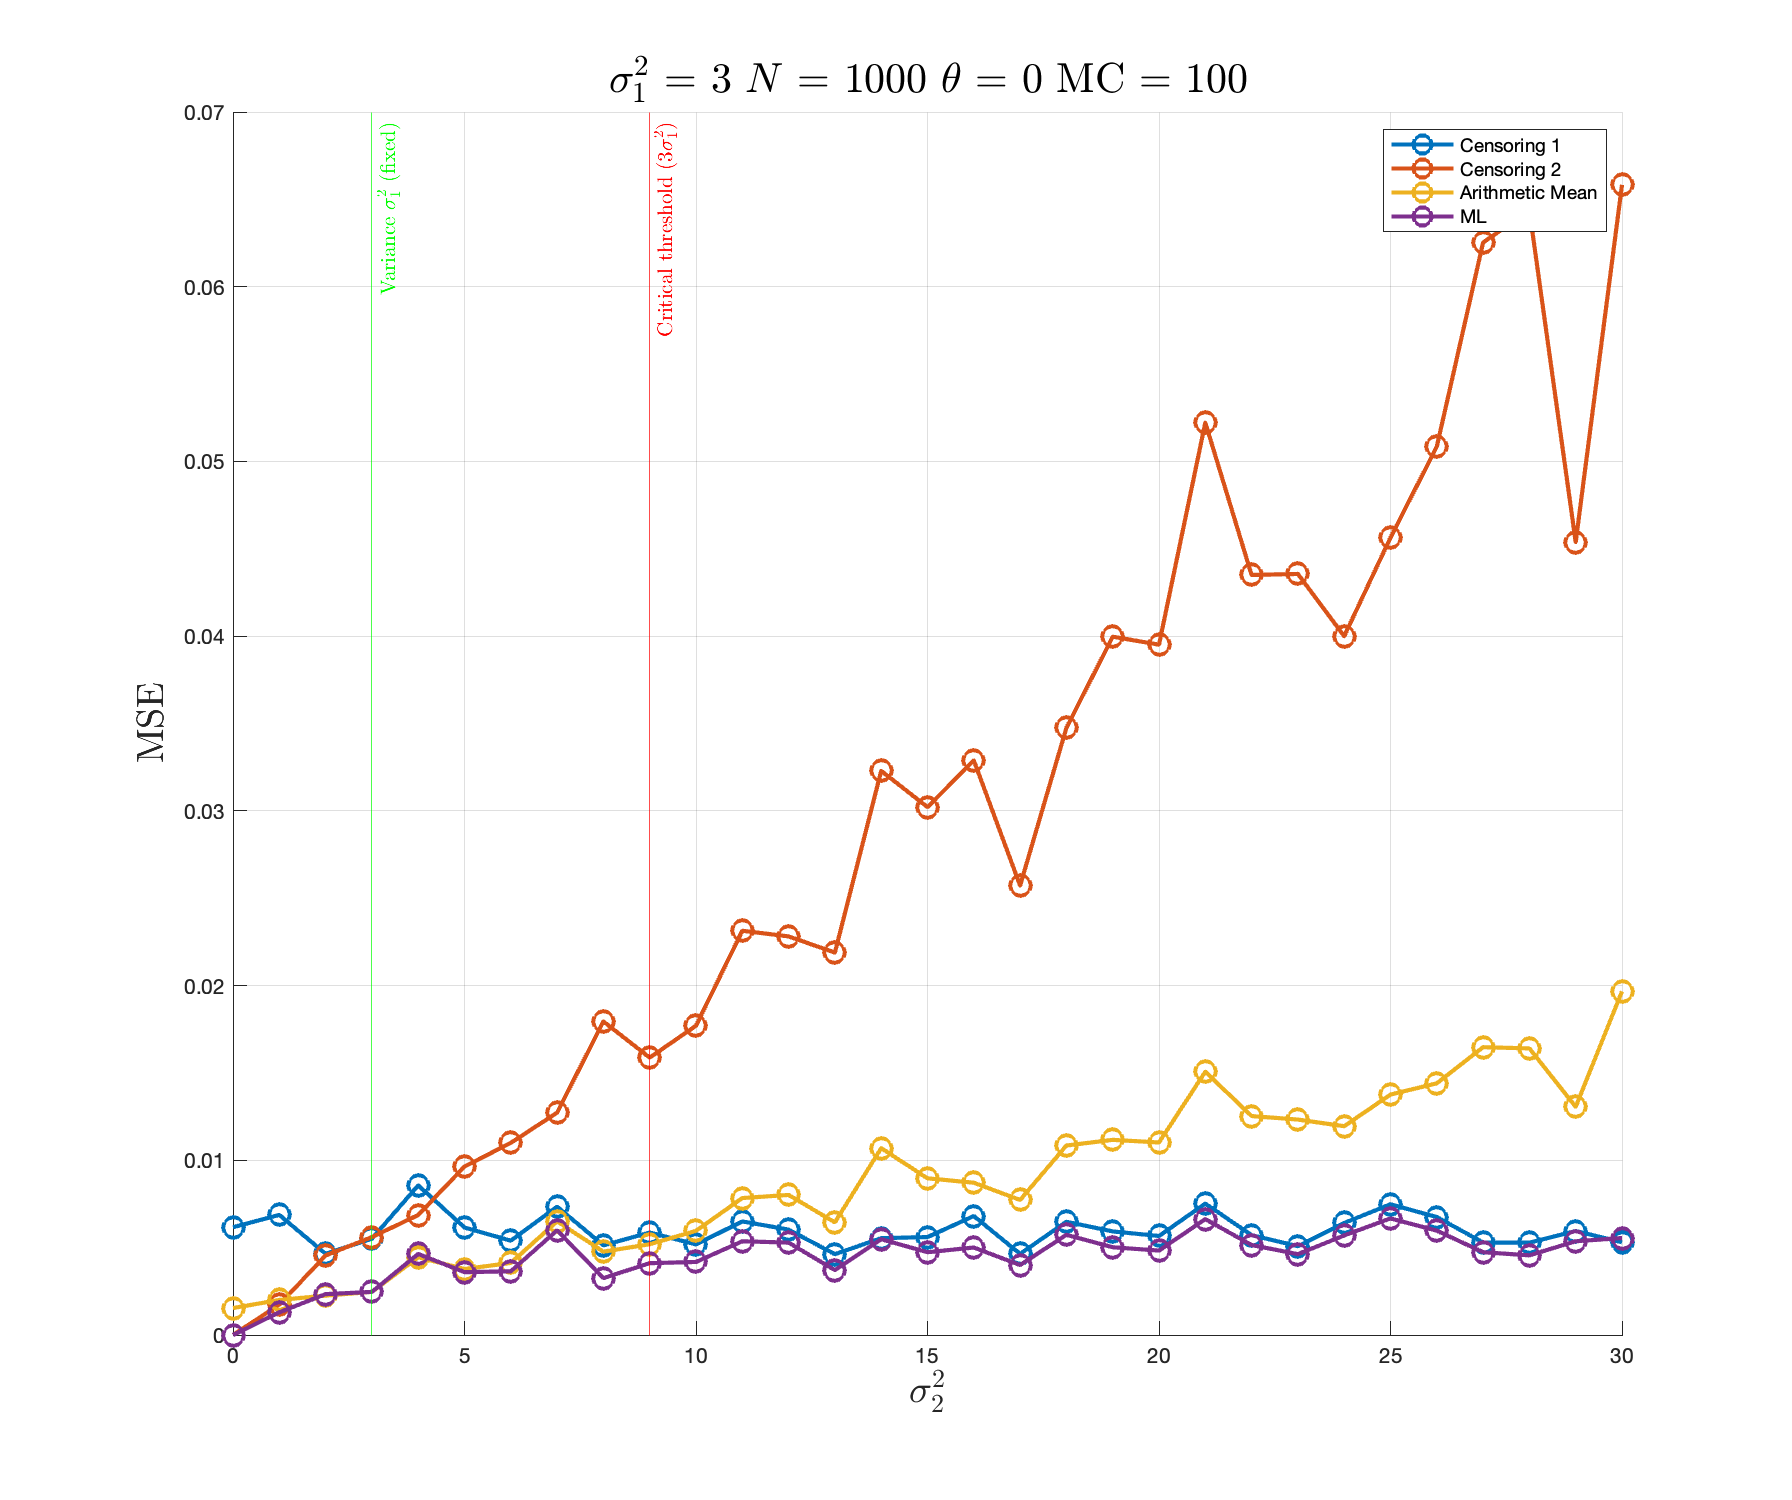
\includegraphics[width=0.8\textwidth]{./figures/appendix_a/figure_1.png}
    \caption{MSE of the estimators $\hat\theta_1$, $\hat\theta_2$, $\hat\theta_{ave}$ and $\hat\theta_{ML}$ as a function of $\sigma_2^2$.}
    \label{fig:mean_estimation_heterogeneous_data}
\end{figure}

Each point is an empirical estimate of the MSE obtained through Monte Carlo simulation, so we will not have exactly the behavior that the theoretical MSE would have, but we are approximating it and this approximation improves by increasing the number of Monte Carlo experiments.

Since we are varying $\sigma_2^2$ we expect the MSE with respect to the estimates made by $\hat \theta _1$ (blue line) to be a constant, remembering however what was said in the first observation to see oscillations is normal being an estimate but increasing $MC$ this approximation can only improve and increasingly resemble a constant.

The MSE shape of $\hat \theta_{ave}$ (yellow line) is increasing as a function of $\sigma^2_2$. It is reasonable since we are adding noise to the system. Since we know the variance of this estimator we also know its theoretical MSE and from it we can observe that the error is linear with respect to $\sigma_2^2$.

From the theoretical analysis we had obtained that there is a special point after which discarding one of the two parts of data is preferable to keeping them equally into account. Therefore, $\hat \theta_{ave}$ (yellow line) which equally weights ($p=0.5$) both parts of data is preferable to $\hat\theta_1$ (blue line) which instead discards completely one part of data (the one that in the graph is increasing its variance) up to this special point which is equal to $3\sigma_1^2$ and represents a level of critical noise for the variance of that slice of data. Beyond this critical point it is preferable to use the estimator $\hat \theta_1$; also from the graph it can be seen how its MSE remains lower than that of $\hat \theta_{ave}$ from the right of the threshold onwards.

It follows that if we wanted to choose between these two the best estimator we would obtain a curve that before the threshold is linear with $\sigma^2_2$ (i.e. $\hat \theta_{ave}$) and after the threshold is a constant, so we would generally have a non-linear behavior as at a certain point there will be a sudden saturation of the error.

The threshold can be read in two different ways depending on whether we vary $\sigma_1^2$ or $\sigma_2^2$.
\[
    \begin{cases}
        \sigma_2^2>3\sigma_1^2 \lor \sigma_1^2<\frac 13\sigma_2^2\quad\text{$\hat\theta_1$ better than $\hat \theta_{ave}$} \\
        \sigma_2^2<3\sigma_1^2\lor \sigma_1^2>\frac13\sigma_2^2\quad\text{$\hat \theta_{ave}$ better than $\hat \theta_1$ }
    \end{cases}
\]

\[
    \begin{cases}
        \sigma_1^2>3\sigma_2^2\lor \sigma_2^2<\frac 13\sigma_1^2\quad\text{$\hat\theta_2$ better than $\hat \theta_{ave}$} \\
        \sigma_1^2<3\sigma_2^2\lor \sigma_2^2>\frac13\sigma_1^2\quad\text{$\hat \theta_{ave}$ better than $\hat \theta_2$ }
    \end{cases}
\]

The MSE computed on the estimates made by $\hat \theta_2$ (red line) increases linearly, as we are inserting more and more noise in that slice of data and therefore we are making the estimate more and more difficult at the same $N$.

The estimator $\hat \theta_{ML}$ with respect to all the other estimators is the best over the entire range of variation as the curve of the MSE calculated on its estimates (purple line) always takes lower values. Only at infinity, it seems to converge with the estimator $\hat \theta_1$ and this is what we would expect from the theory.
If we didn't have any formula to support and therefore we should rely only on the data and the simulation we could never be firmly convinced that the MSE of $\hat\theta_{ML}$ is always better than $\hat \theta_1$ as they are too close and it could be just a case that the purple line is lower over the entire range (as experiments we could never be sure). What we could do in a situation like this is:
\begin{enumerate}
    \item Do experiments with different orders of magnitude for the number of Monte Carlo simulations and see if there is a common trend
    \item If at the same data, the curves are very irregular and despite this there is a curve that always has lower values than another, it could be a clue that this phenomenon is also true in theory
\end{enumerate}
When $\sigma_1^2=\sigma_2^2$ the two points of the two curves of the MSE of $\hat\theta_1$ and $\hat\theta_2$ assume the same identical value. The same value for the curves of $\hat\theta_{ML}$ and $\hat\theta_{ave}$ because the weights given by the ML estimator are equal to those implicit in the arithmetic mean ($p=0.5$).
When $\sigma_2^2=0$ we have a slice of data that is giving us exactly the value of the unknown parameter $\theta$, and therefore the MSE of $\hat\theta_2$ will clearly be $0$. In this particular circumstance the performance of $\hat\theta_2$ is equal to that of $\hat\theta_{ML}$.
When $\sigma_2^2\to+\infty$ the ML estimator will tend to give less and less weight to that slice of data as it becomes more and more noisy and therefore asymptotically the performance of $\hat\theta_{ML}$ will be equal to those of $\hat \theta_1$ and in particular will converge to a certain value.

The two previous points show the boundaries of the performance of the ML estimator. In both cases there is a fixed variance, and there is a variance that dominates the other. In one case we have $\sigma_1^2$ fixed and dominated by $\sigma_2^2$, so the slice of data with variance $\sigma_2^2$ becomes "optimal" and the ML estimator moves in that direction. Conversely in the second case $\sigma_1^2$ is still fixed but dominated by $\sigma_2^2$ which in this case indicates that its part of data is becoming worse, so the ML estimator directs its estimates based on the "best" slice of data.

The arithmetic mean cannot guarantee the behavior of the previous point because it does not take into account the parameters so regardless of the value that the variance continues to take information in the same way from both slices of data.

Taking the three estimators $\hat\theta_{ave}$, $\hat\theta_{1}$ and $\hat\theta_{2}$ the curve obtained by properly selecting the best of them at each point is not so different from the curve of $\hat \theta_{ML}$.

\begin{figure}[H]
    \centering
    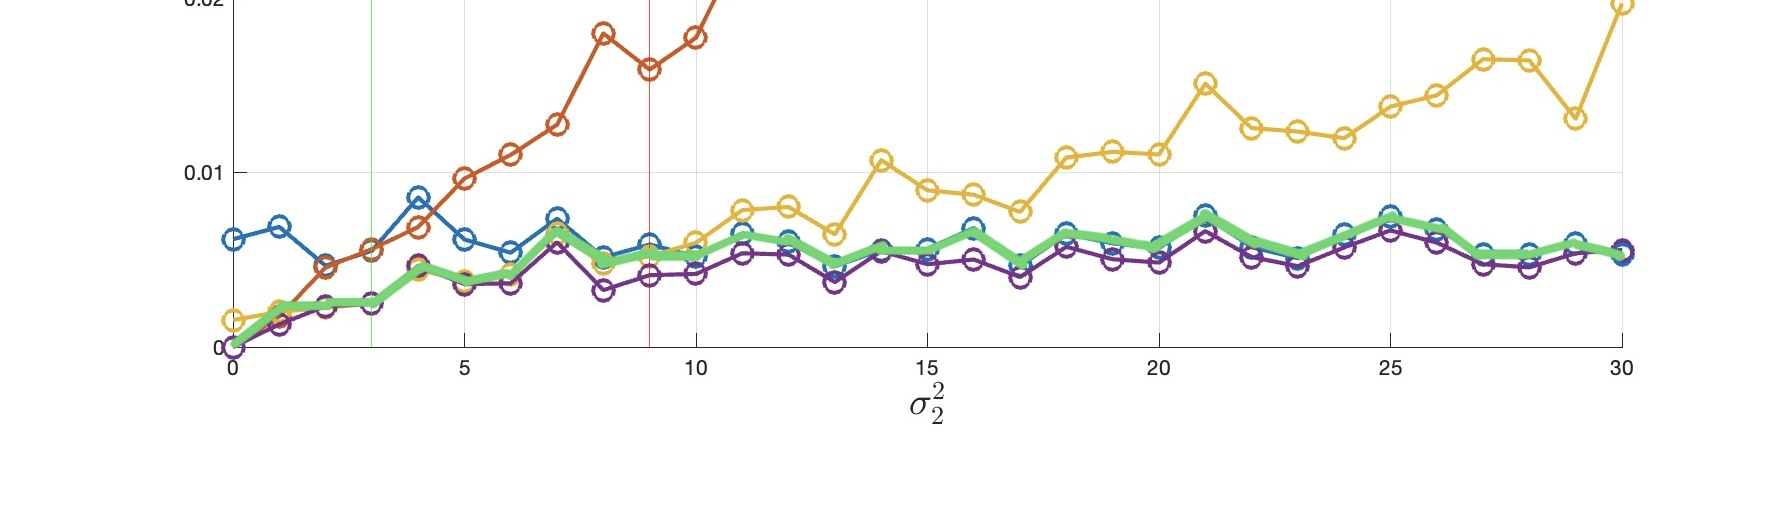
\includegraphics[width=\textwidth]{./figures/appendix_a/figure_2.jpeg}
\end{figure}

Let us observe the comparison between the theoretical error (corresponding to the variance as we have previously said) and the estimated MSE.

\begin{figure}[H]
    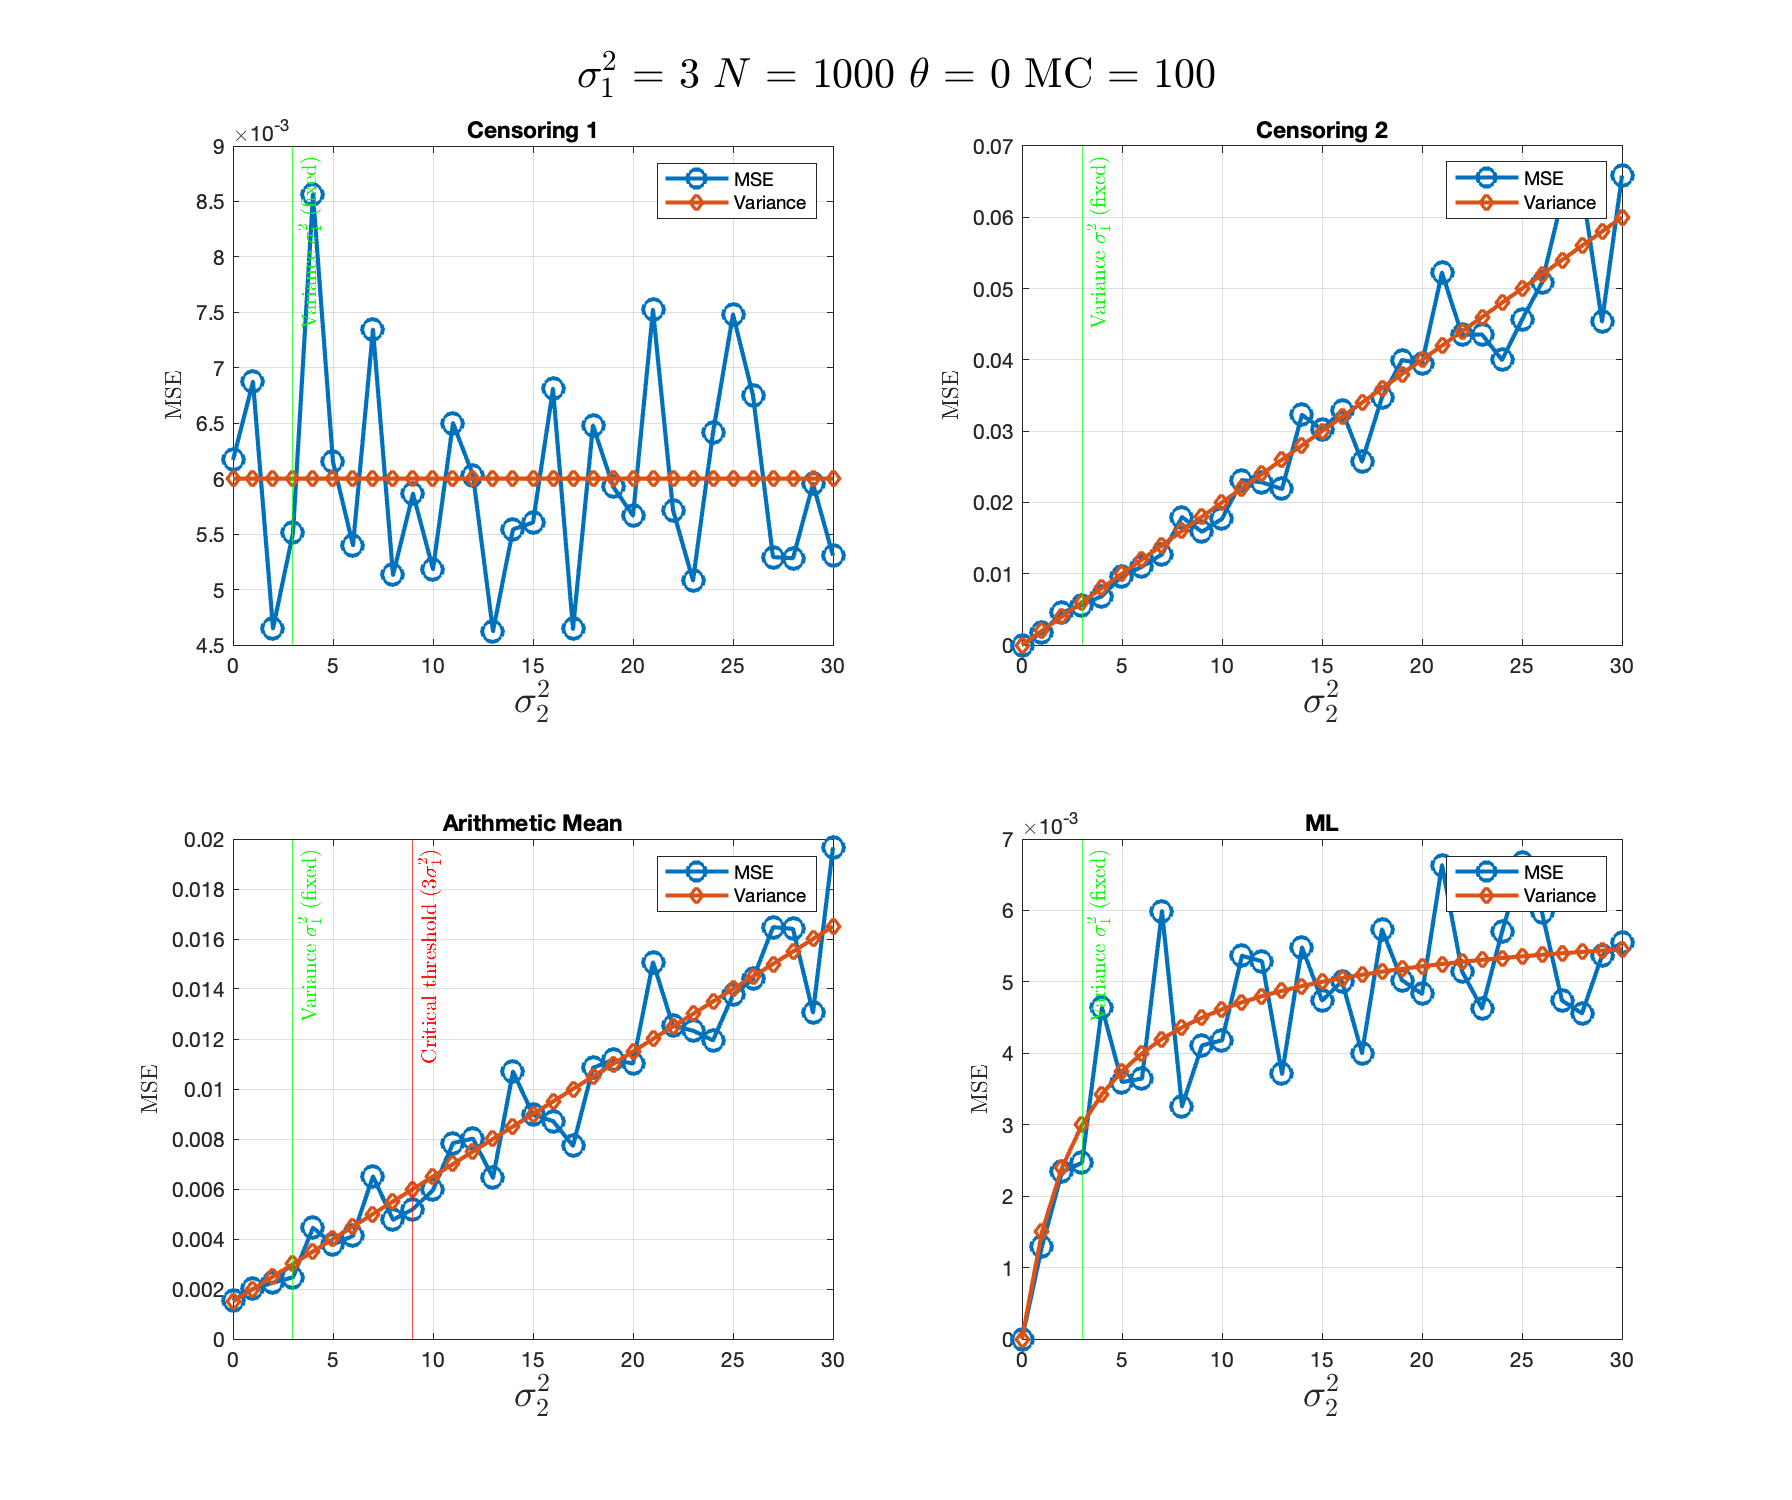
\includegraphics[width=\textwidth]{./figures/appendix_a/figure_3.png}
\end{figure}

\textit{If I have more noise the error is greater and in fact we have seen how increasing the variance increases the error in general. But if I want to estimate that error with the Monte Carlo simulation, with noisier data it is more complex to make the estimate?}

The answer is clearly yes, if I have noisier data everything seems more random and therefore I need more simulations. Let us observe what happens if we increase the number of simulations by an order of magnitude.

\begin{figure}[H]
    \centering
    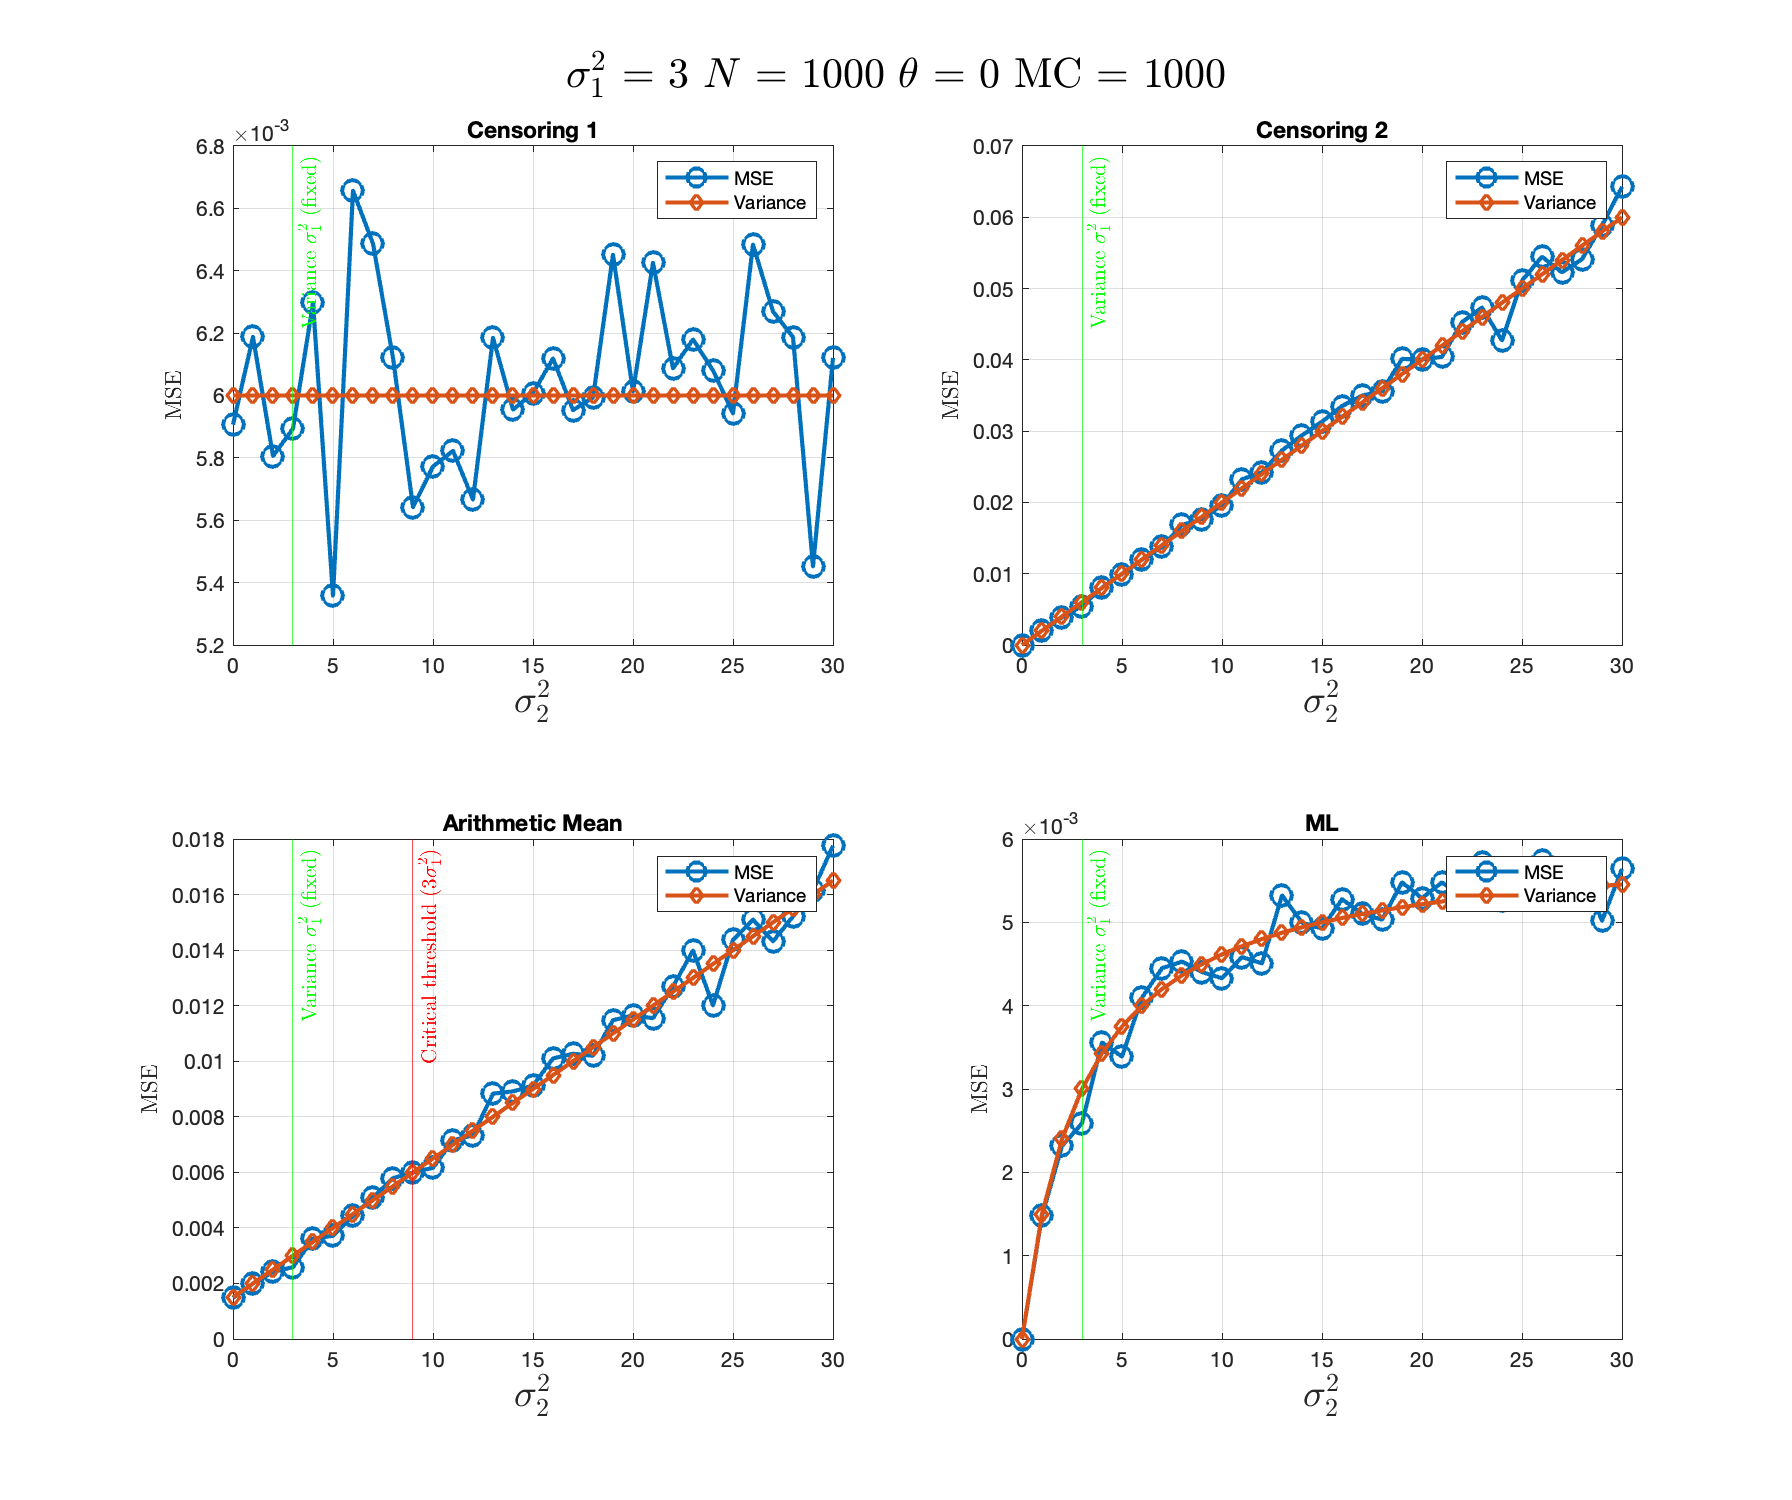
\includegraphics[width=\textwidth]{./figures/appendix_a/figure_4.png}
\end{figure}

\subsection*{Variation of $N$}

Let's look at the variation of the MSE as $N$ increases, both using a linear scale for the y-axis and a logarithmic scale. We also perform a comprehensive analysis from the perspective of the two scenarios we could encounter: $\sigma_2^2>3\sigma_1^2$ and $\sigma_2^2\le3\sigma_1^2$.

We can observe that using both logarithmic scales, the curve has a linear trend. This means that the actual trend is a power of $N$, specifically in this case $N^{-1}$. All these curves decrease with the same law (\textbf{scaling law}, often a theoretical result is expressed in terms of it). This is also derived from theory as the theoretical error decreases proportionally to $N$.

\begin{note}{About scaling laws}
    A scaling law is
    $$
        y=a\cdot x^b
    $$

    If we used a logarithmic scale to represent this relationship we would have:
    $$
        \log(y)=\log(a\cdot xb)=\log(a)+b\cdot\log(x)
    $$

    Since increasing $x$ the curve decreases with a unit slope, the value of $b=-1$, net of the proportionality coefficient $a$ which is different for all the curves.
\end{note}
\begin{note}{Comparison between scaling laws}
    For this type of problems $\frac 1N$ is the best scaling law we could have in an independent sample estimation problem. So an estimator with this scaling law can be considered a good estimator, although the constant may then make the difference between estimators with the same scaling law.
    Only in extremely particular cases can we have exponential scaling laws.
\end{note}

The estimator $\hat\theta_{ML}$ not only has a scaling law of $\frac 1N$, but also has a smaller constant compared to the other estimators. In fact, we can observe that its curve is lower than the others.

We notice that in the two cases, respectively to the right and to the left of the threshold on the variance that emerged from the theory, we have a different ordering of the curves of $\hat\theta_{ave}$ and $\hat \theta_1$.


\section{MMSE}
In this exercise, we are going to use Monte Carlo simulations to verify the theoretical results obtained in section \ref{sec:ex_2}. The minimum mean square error for a random variable $Y$ given a set of observations $X$ is:
\[
    \hat{Y} = \E{}{Y\mid X} = \frac{\sigma^2_y}{\sigma^2_y + \frac{\sigma^2_w}{N}} \bar{X}
\]
While its variance is:
\[
    Var[Y|X]=\frac {\sigma^2_Y\sigma^2_W}{\sigma^2_W+N\sigma^2_Y}
\]

%TODO: Restore table
In table \ref{tab:mmse} we can see the theoretical values of the MMSE varying $\sigma^2_W$ and $\sigma^2_Y$.

\begin{table}[H]
    \centering
    \begin{tabular}{|c|c|c|}
        \hline
        $\lim$                 & $\alpha$ & $MMSE$      \\
        \hline
        $\sigma^2_Y\to+\infty$ & $1$      & $\bar X$    \\
        $\sigma^2_Y\to 0$      & $0$      & $0 (\mu_Y)$ \\
        $\sigma^2_W\to+\infty$ & $0$      & $0$         \\
        $\sigma^2_W\to 0$      & $1$      & $\bar X$    \\
        \hline
    \end{tabular}
    \quad
    \begin{tabular}{|c|c|c|}
        \hline
        $\gg$          & $\sigma^2_W/N$     & $\sigma^2_Y$                                   \\
        \hline
        $\sigma^2_W/N$ & -                  & $\alpha \approx \frac{\sigma^2_Y}{\sigma^2_W}$ \\
        $\sigma^2_Y$   & $\alpha \approx 1$ & -                                              \\| $\lim$ | $\alpha$ | $MMSE$ |
    \end{tabular}
\end{table}

\subsection*{Variation of $\sigma^2_Y$}
Let's first consider the case where $\sigma^2_Y$ is much larger than $\frac {\sigma^2_W}N$.

\begin{figure}[H]
    \centering
    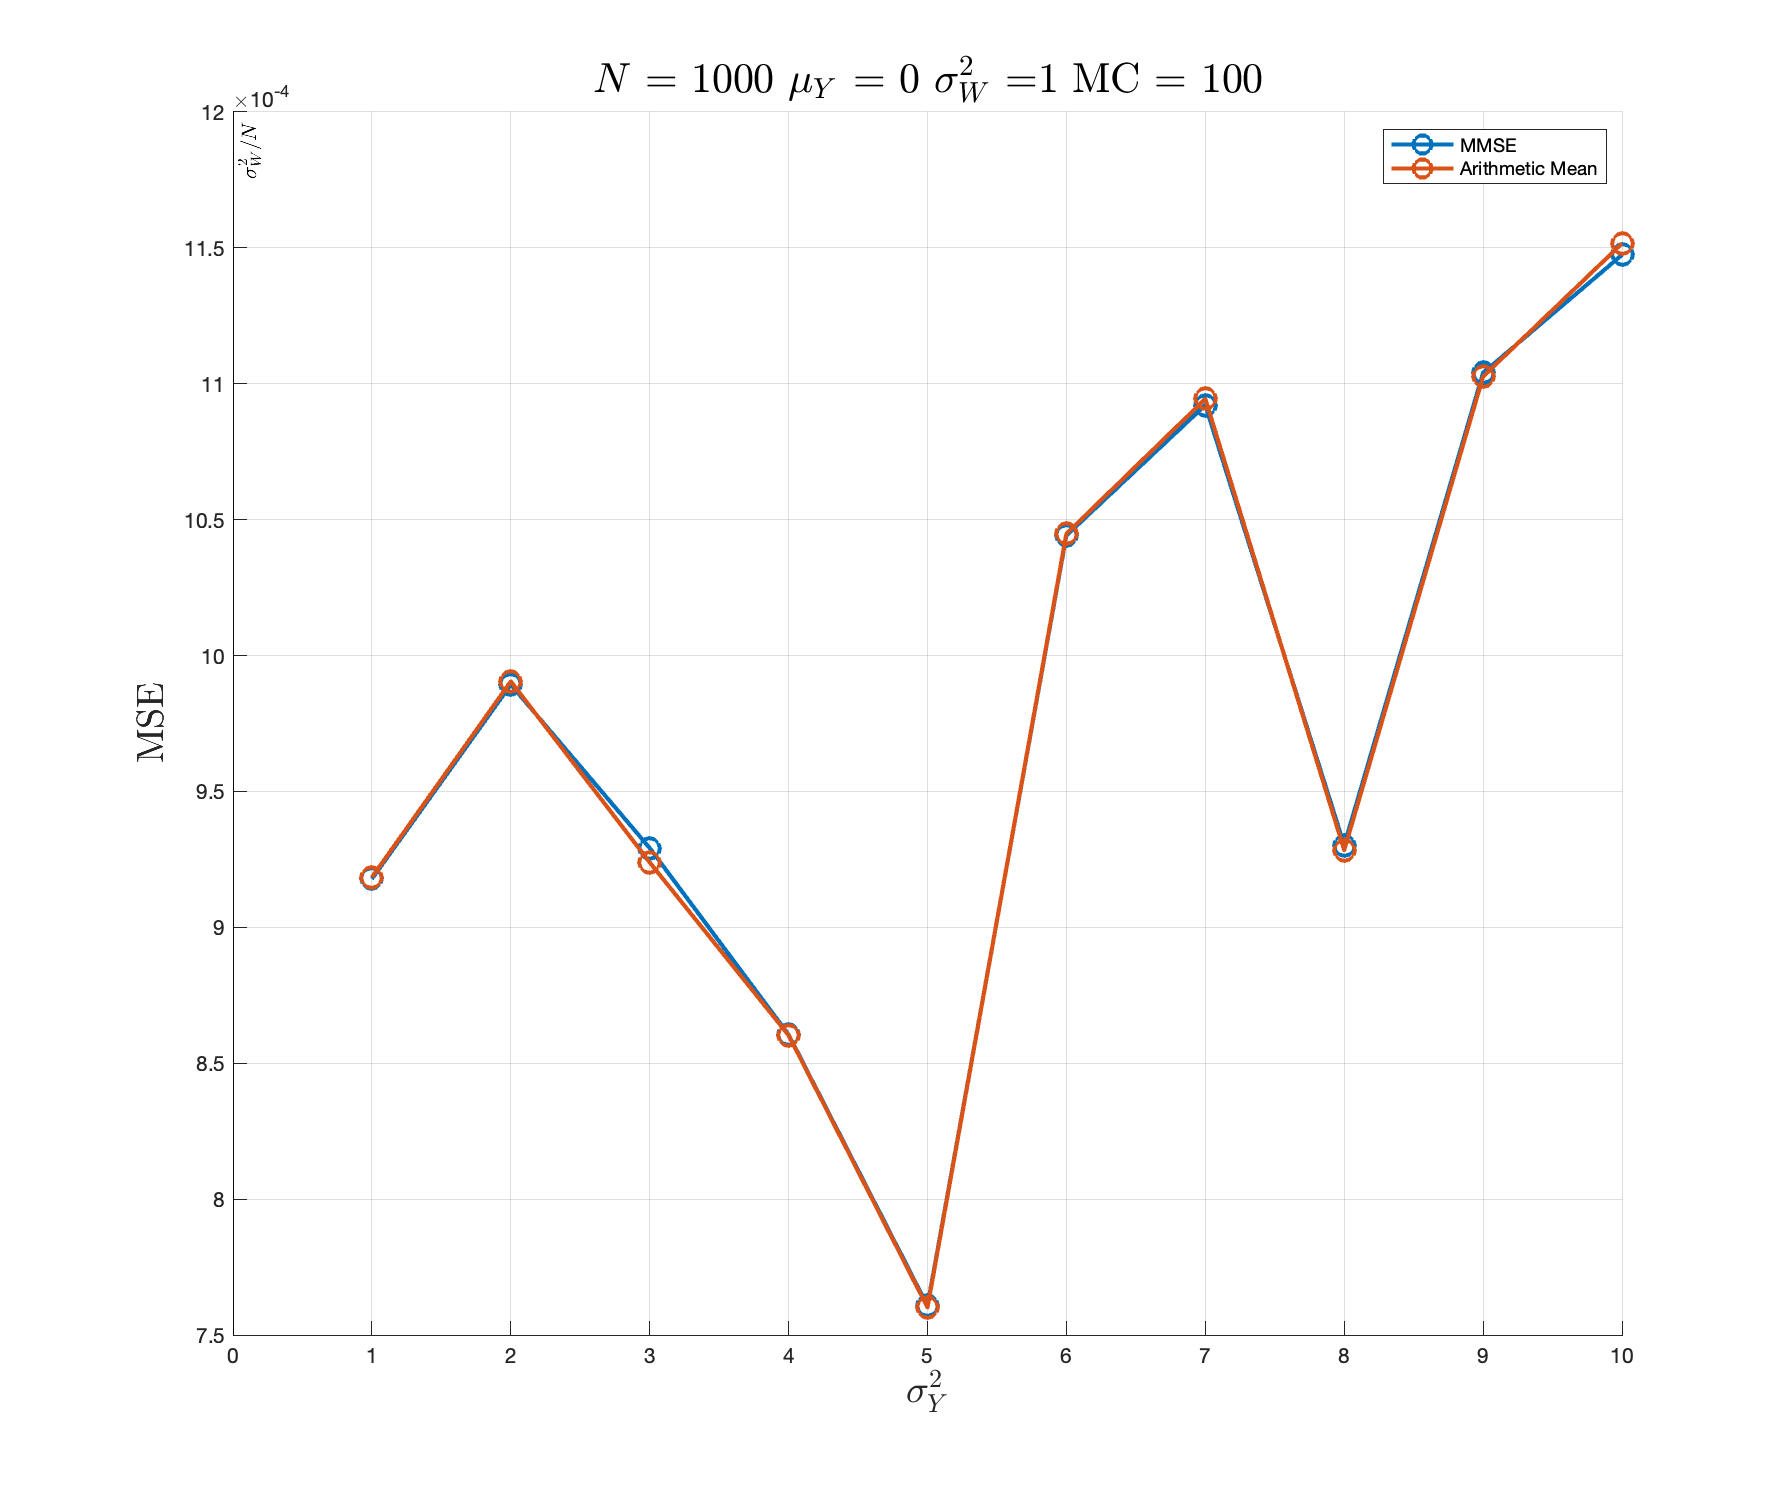
\includegraphics[width=0.8\textwidth]{./figures/appendix_a/figure_6.png}
    \caption{MSE of the estimators $\hat Y$ and $\bar X$ as a function of $\sigma^2_Y$.}
    \label{fig:mmse_sigma_y}
\end{figure}

As in the theoretical analysis, we can observe that when the variance of the prior function is much larger than the ratio between the variance of the error and the number of samples, the two estimators tend to behave in the same way. In fact, in this case, $\alpha\to 1$ and the MMSE tends to the arithmetic mean.

Also as expected, if we did not have data (or equivalent data that is independent of $Y$), but only the information of the prior distribution, the MMSE would be the mean of the prior distribution.

$$
    \mathbb E[Y|X]=\mathbb E[Y]=\mu_Y
$$
in that case the MSE would be:
$$
    \mathbb E[(Y-\hat Y)^2]=Var[Y]=\sigma_Y^2
$$
So we can see this result as a upper bound to the error we can obtain.
% TODO: controllare le caption delle immagini
Having  $\sigma^2_Y \gg \frac{\sigma^2_W}N$ the information we have from the prior distribution is not very informative. Having an high variance of the parameter means saying that the parameter may be everywhere in the domain, so it makes sense that the MMSE can work as the arithmetic mean since the only information we have are the data.
\begin{figure}[H]
    \centering
    \begin{minipage}{0.45\textwidth}
        \centering
        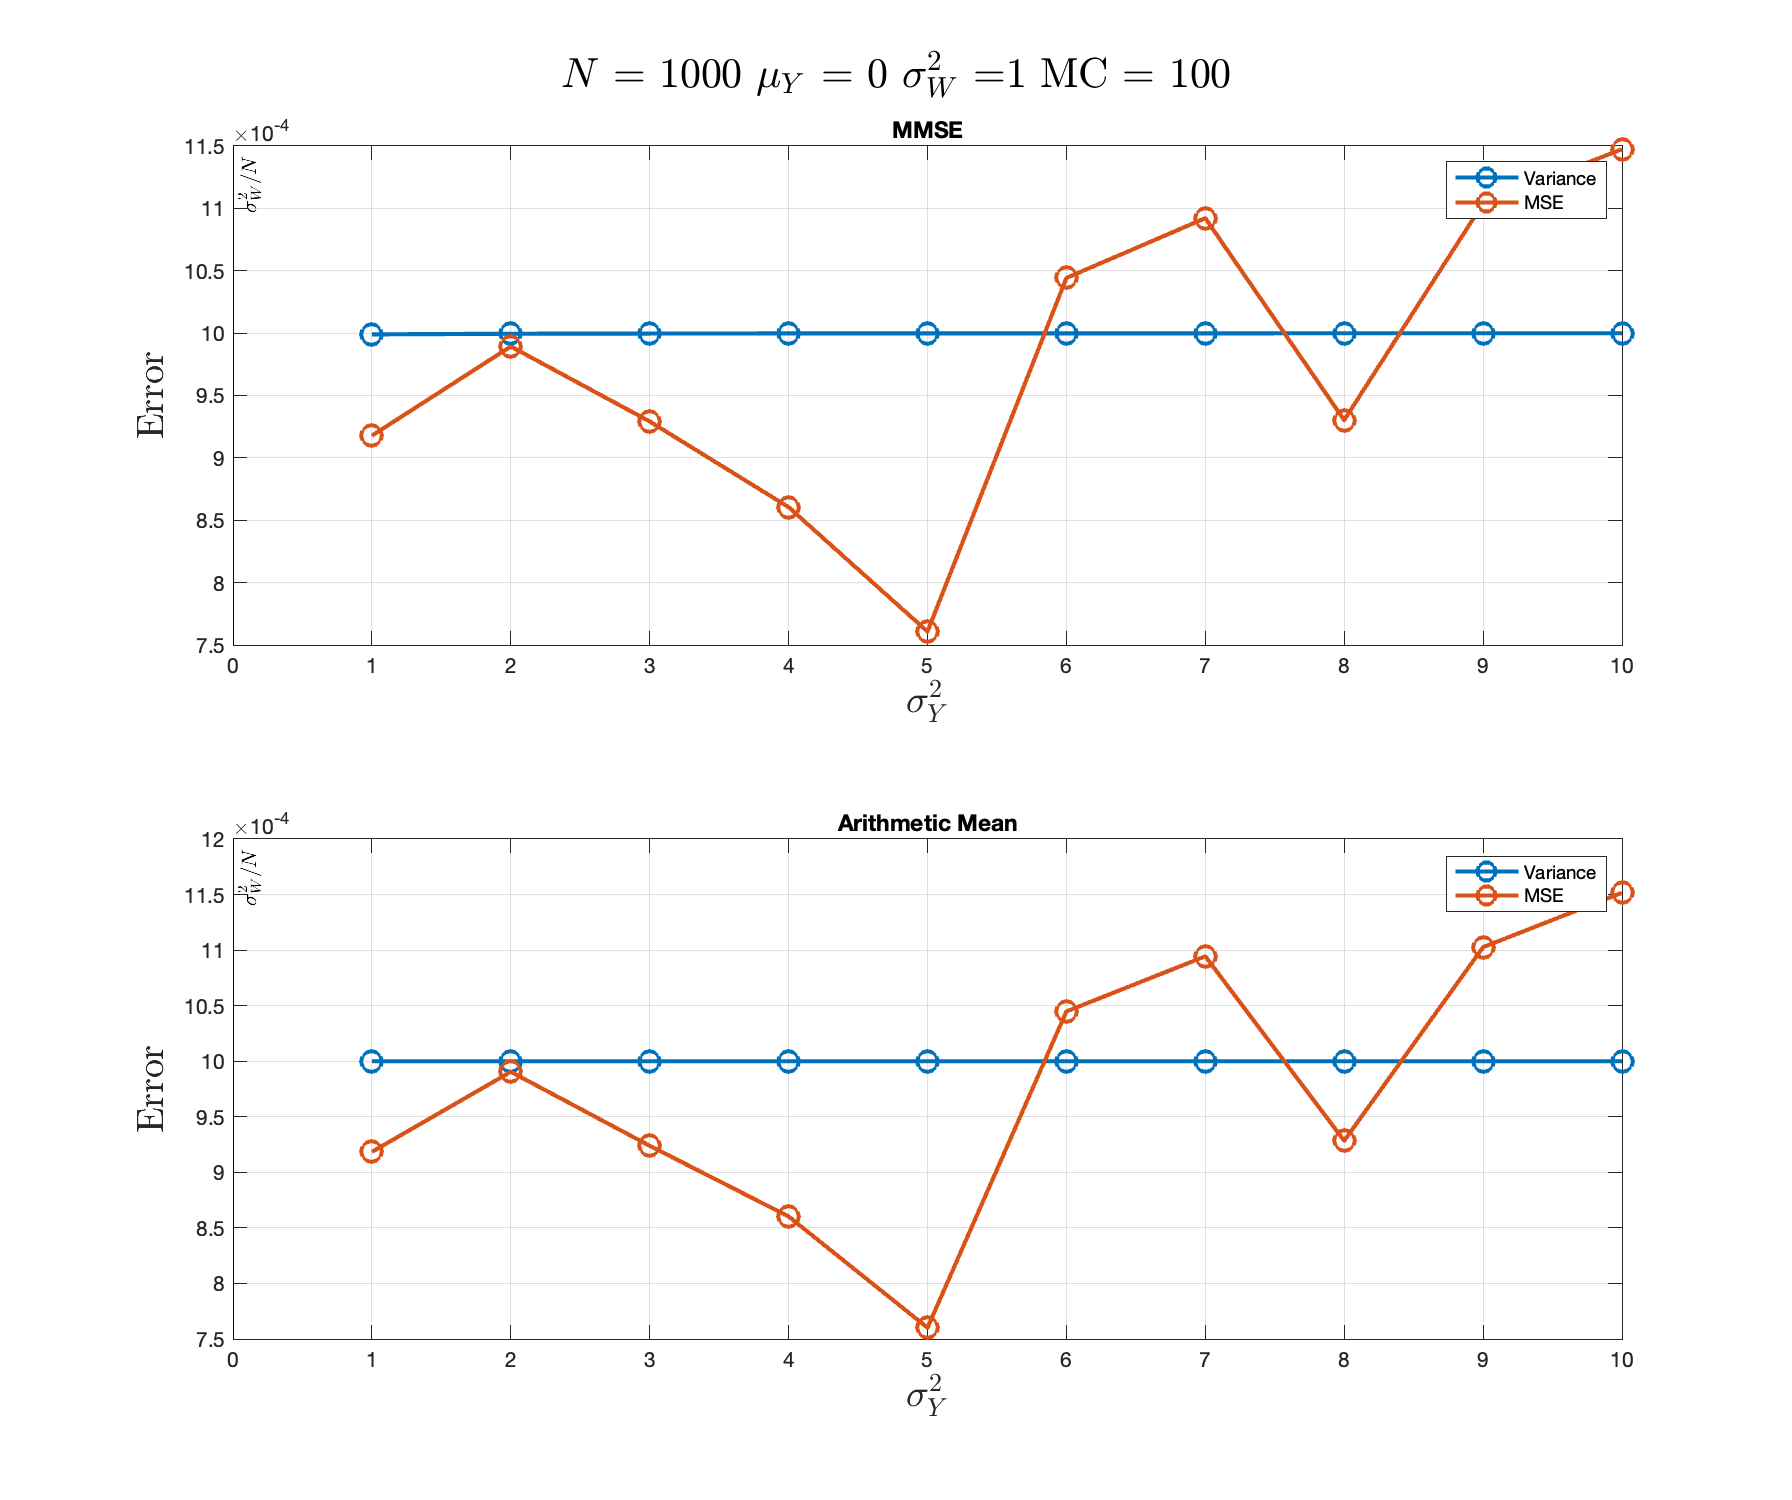
\includegraphics[width=\textwidth]{./figures/appendix_a/figure_7.png}
    \end{minipage}
    \hfill
    \begin{minipage}{0.45\textwidth}
        \centering
        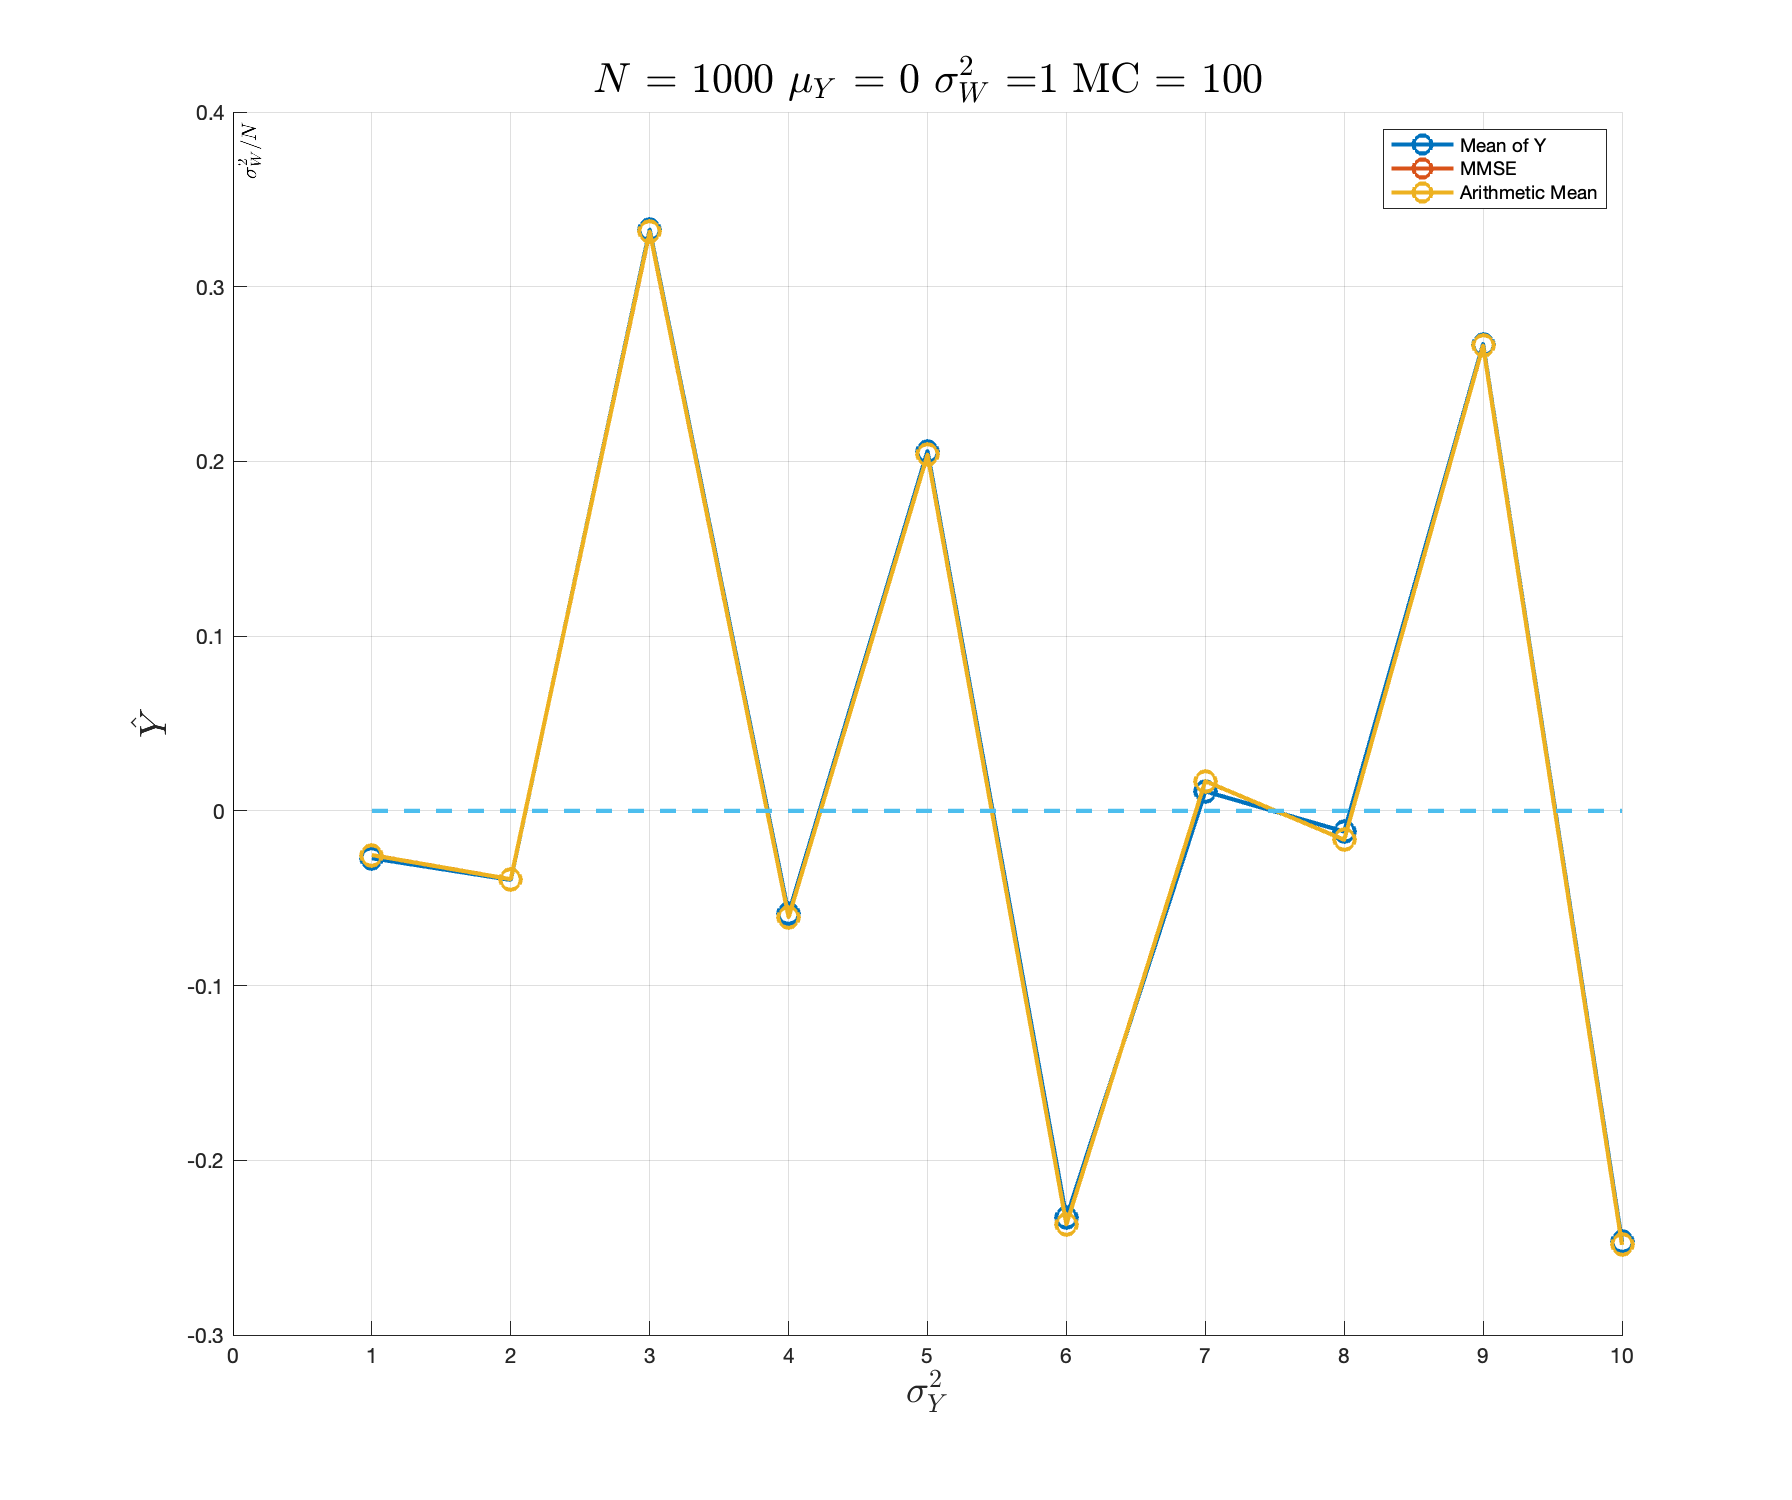
\includegraphics[width=\textwidth]{./figures/appendix_a/figure_8.png}
    \end{minipage}
    \caption{MSE of the estimators $\hat Y$ and $\bar X$ as a function of $\sigma^2_Y$.}
    \label{fig:mmse_sigma_y_combined}
\end{figure}

Let's now consider the case where $\sigma_Y^2$ is much smaller than $\frac {\sigma^2_W}N$.

\begin{figure}[H]
    \centering
    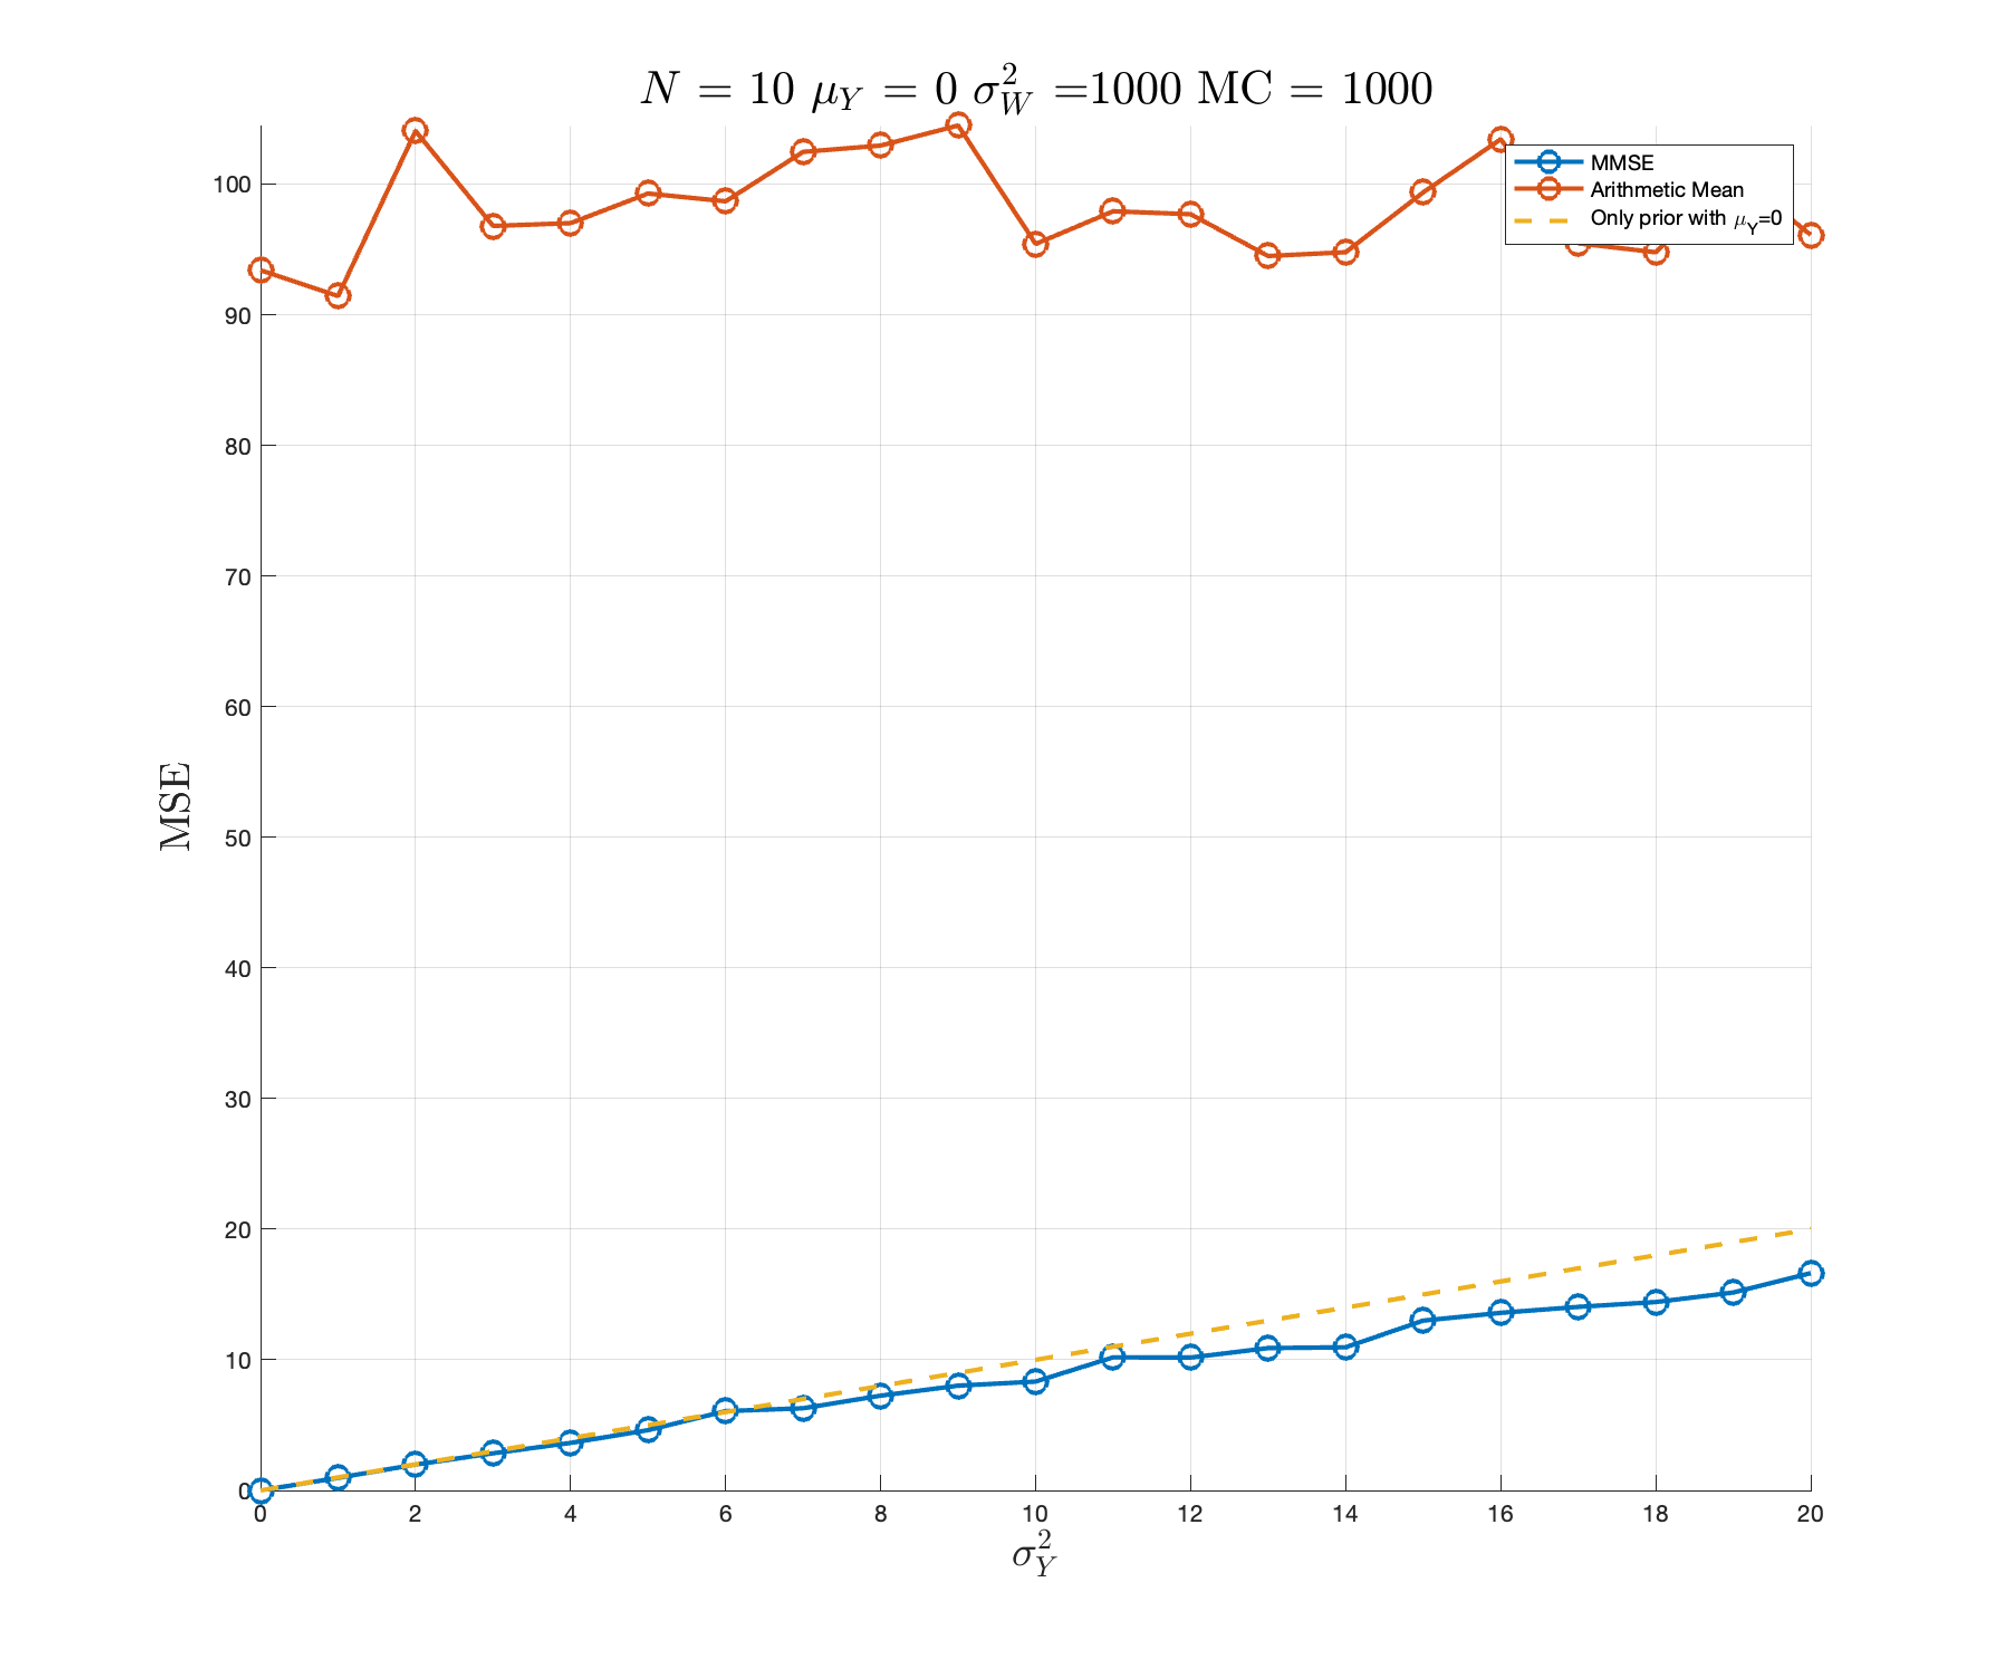
\includegraphics[width=0.8\textwidth]{./figures/appendix_a/figure_9.png}
    %\caption{MSE of the estimators $\hat Y$ and $\bar X$ as a function of $\sigma^2_Y$.}
    %\label{fig:mmse_sigma_y_small}
\end{figure}

\begin{figure}[H]
    \centering
    \begin{minipage}{0.45\textwidth}
        \centering
        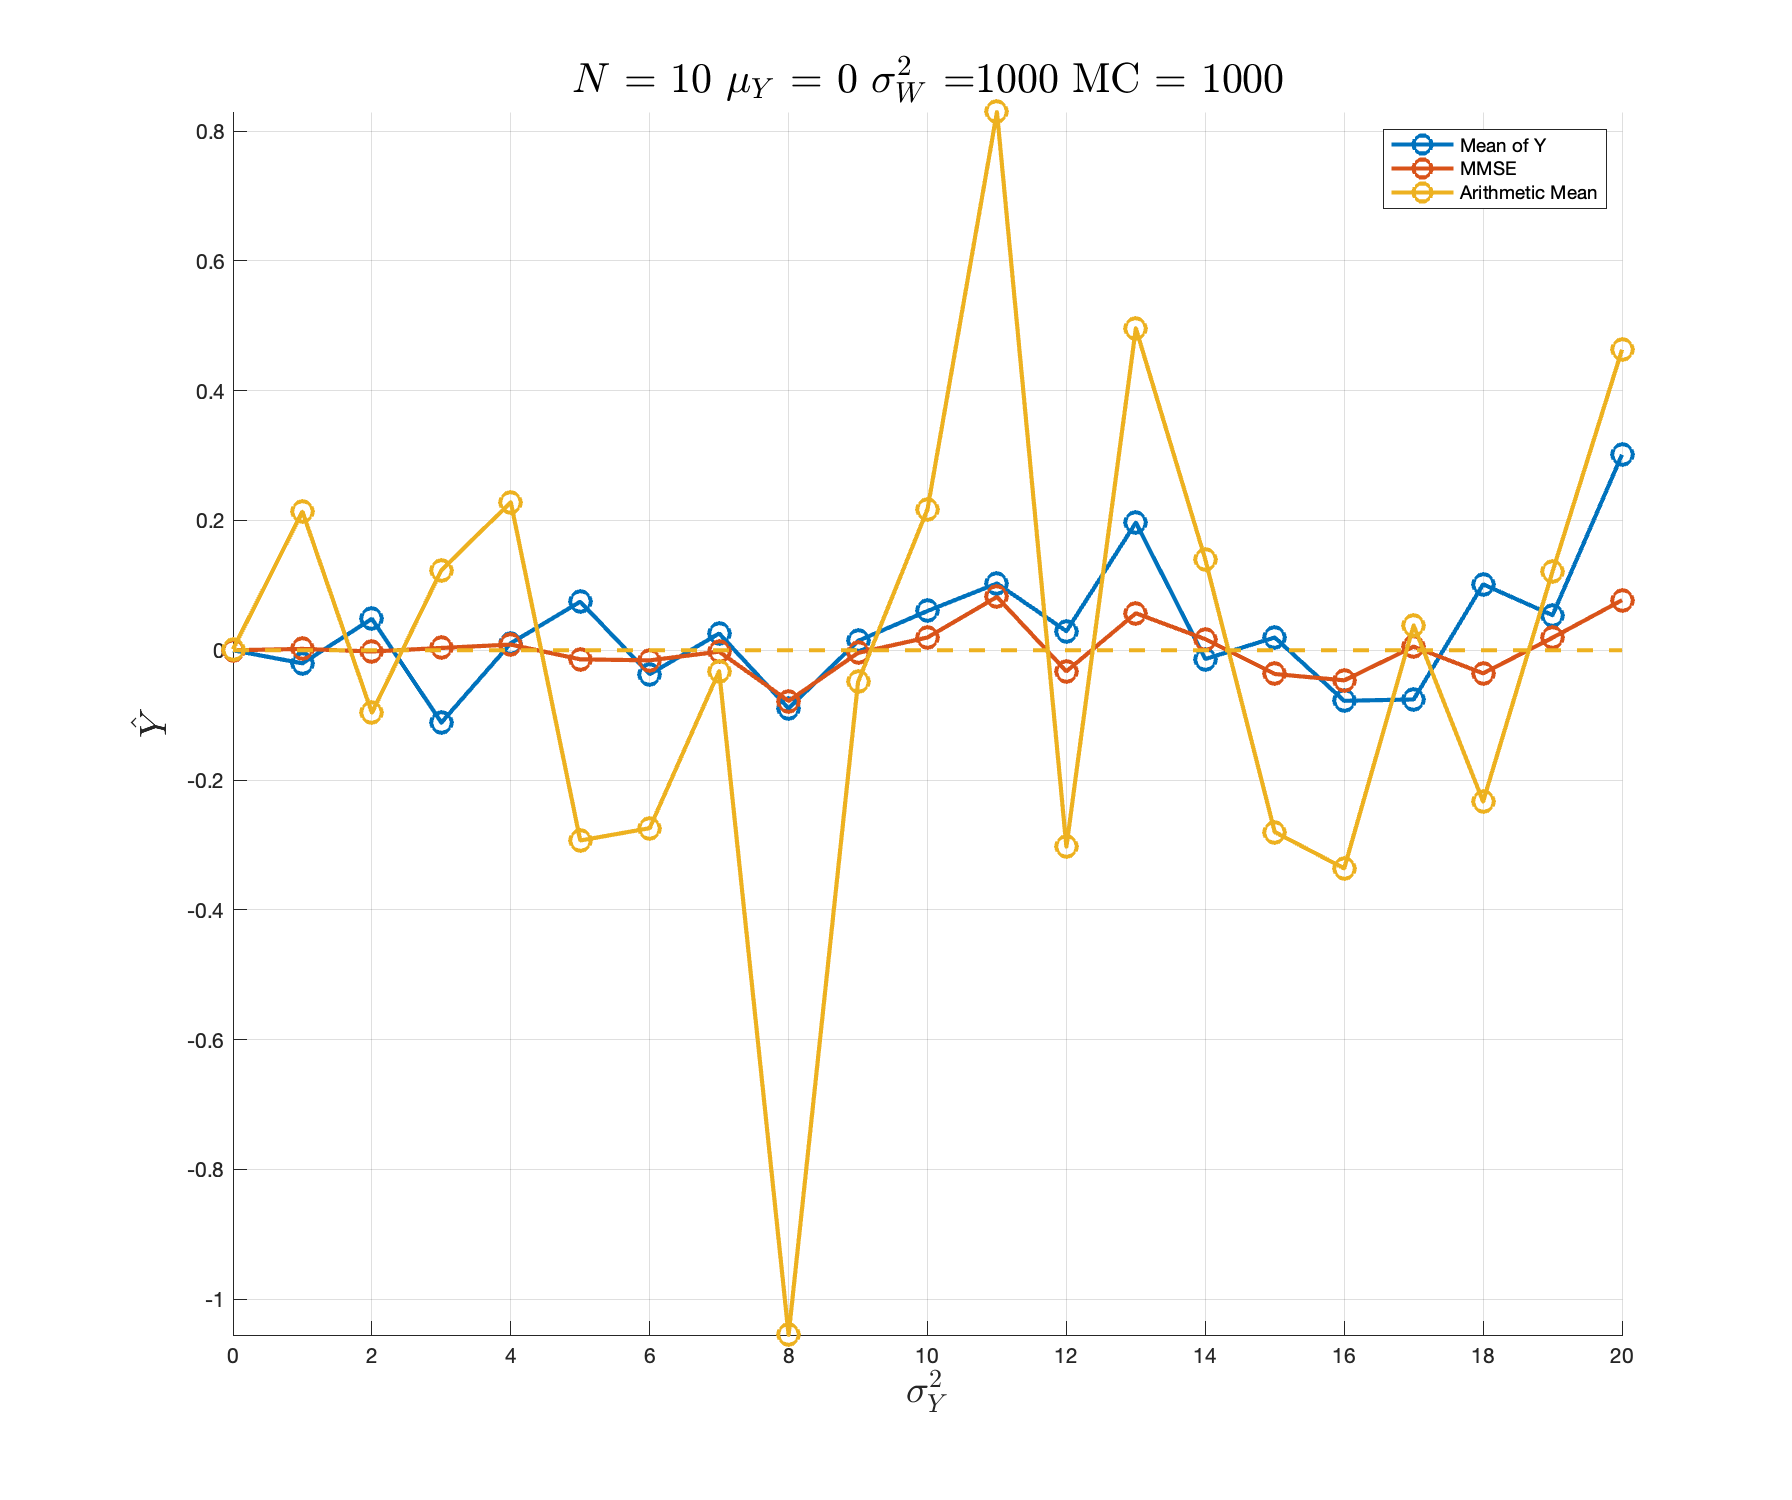
\includegraphics[width=\textwidth]{./figures/appendix_a/figure_10.png}
    \end{minipage}
    \hfill
    \begin{minipage}{0.45\textwidth}
        \centering
        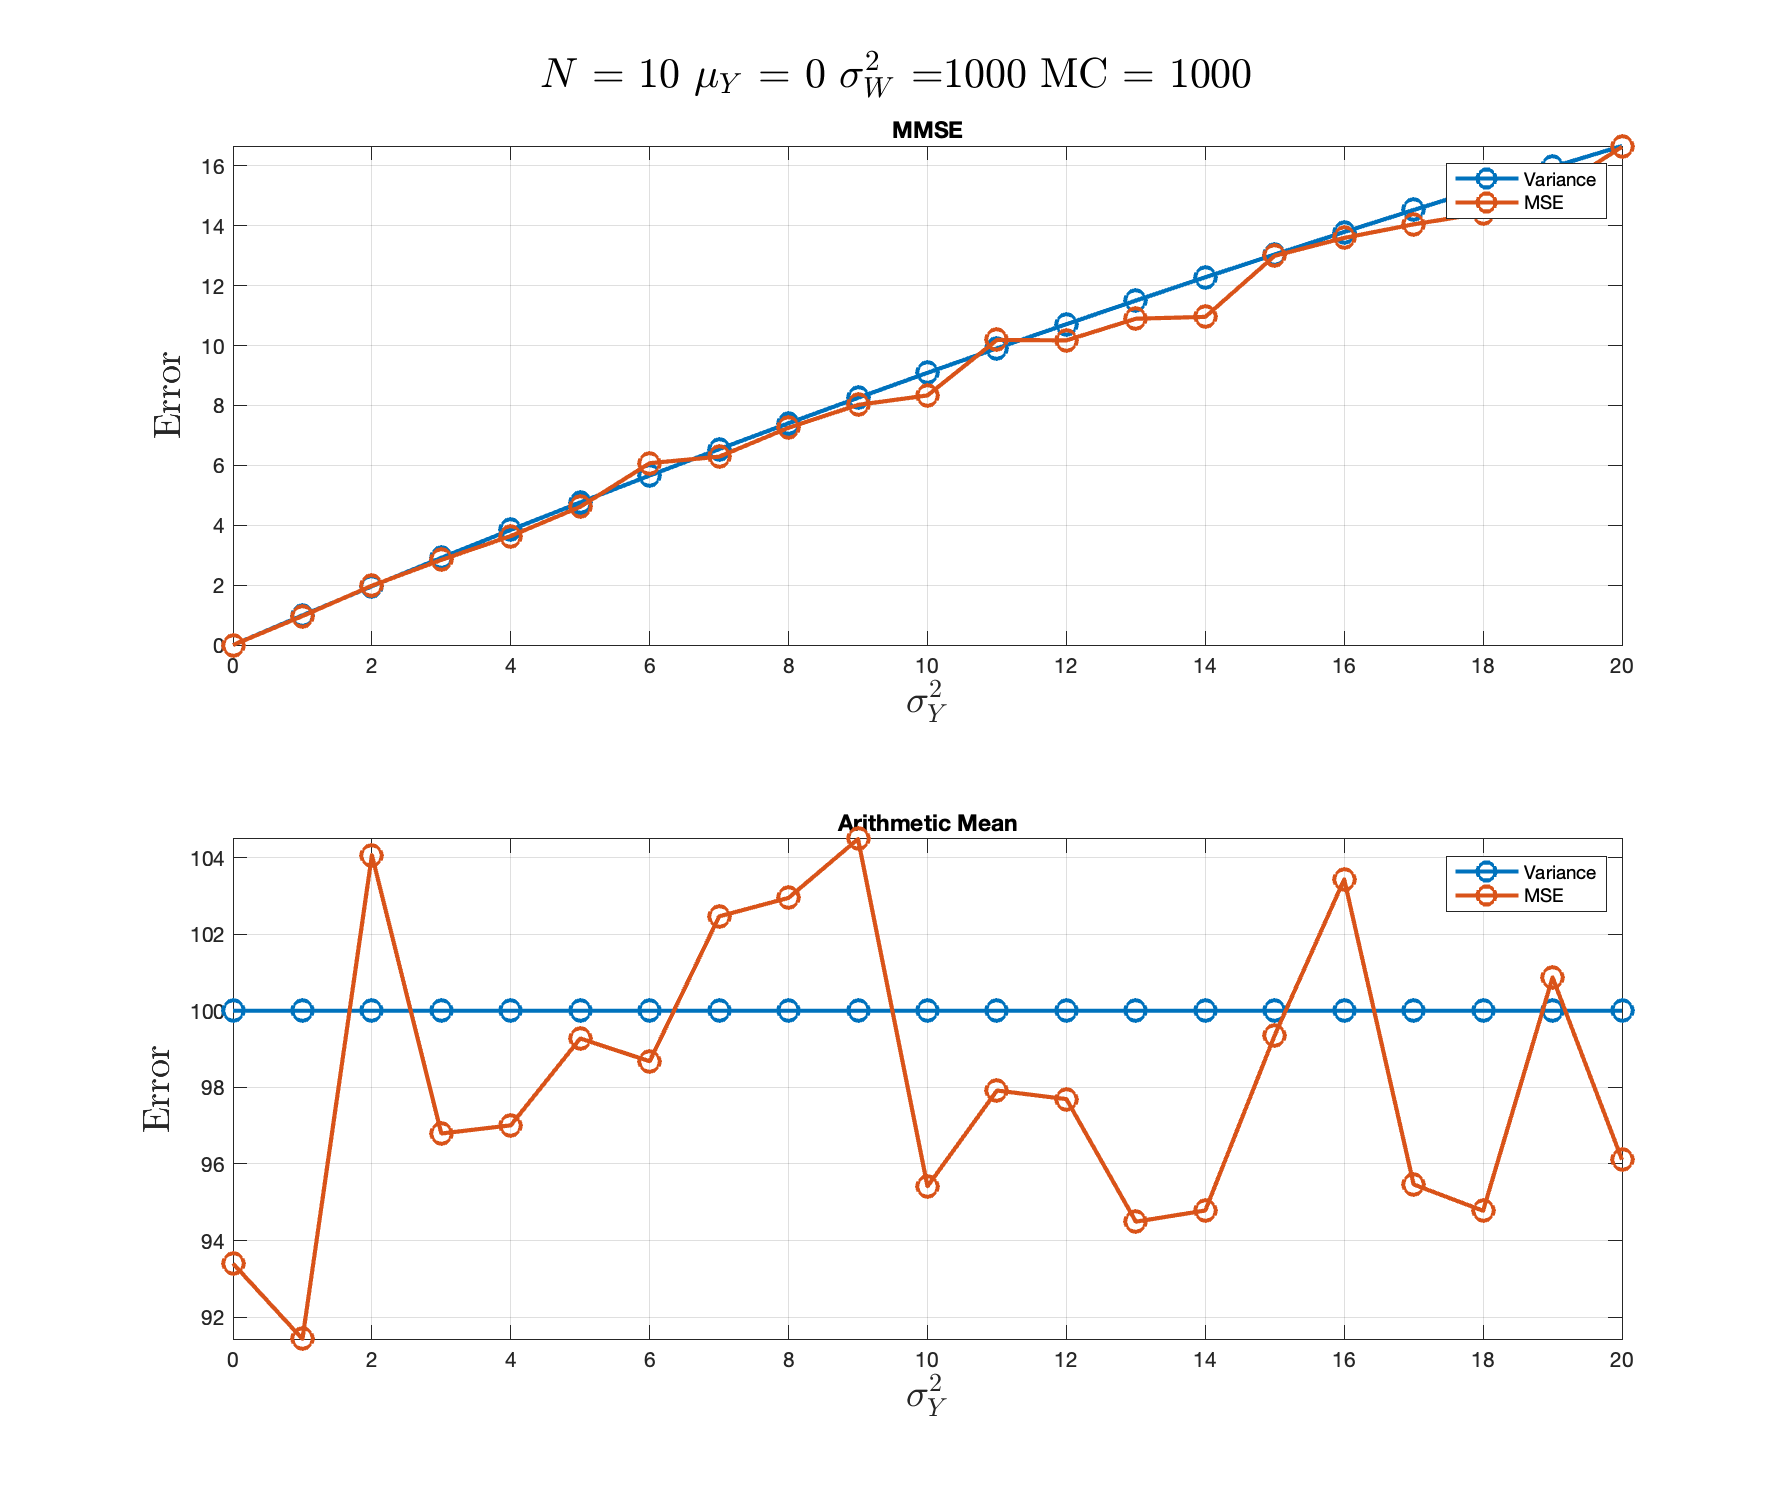
\includegraphics[width=\textwidth]{./figures/appendix_a/figure_11.png}
    \end{minipage}
    %\caption{MSE of the estimators $\hat Y$ and $\bar X$ as a function of $\sigma^2_Y$.}
    %\label{fig:mmse_sigma_y_combined}
\end{figure}

\begin{enumerate}
    \item The data is very noisy compared to the prior information we have. In fact, the posterior mean performs better on average than the arithmetic mean.
    \item In the extreme case, when this difference is quite pronounced, we are making an estimation based solely on the prior information. In fact, the estimates made by the MMSE are practically a constant at $0$.
    \item The MMSE estimator is infused with prior information. To understand if this information leads to better results compared to completely eliminating the data using the estimator $\hat Y=0$ and plotting the value of $\mathbb E [Y^2]$, which is equal to $\sigma^2_Y$ since $\mu_Y=0$ (yellow dashed line added afterwards).
          Noticing that the MSE always stays below this bisector and has a sublinear growth, we can appreciate that using data infused with prior information yields beneficial results and will eventually converge to the error of the arithmetic mean (not visible in these plots but in those for $\sigma^2_Y\gg \frac{\sigma^2_W}{N}$).
\end{enumerate}

Now, let's consider the case where $\sigma^2_Y$ is comparable to $\frac {\sigma^2_W}N$.

\begin{figure}[H]
    \centering
    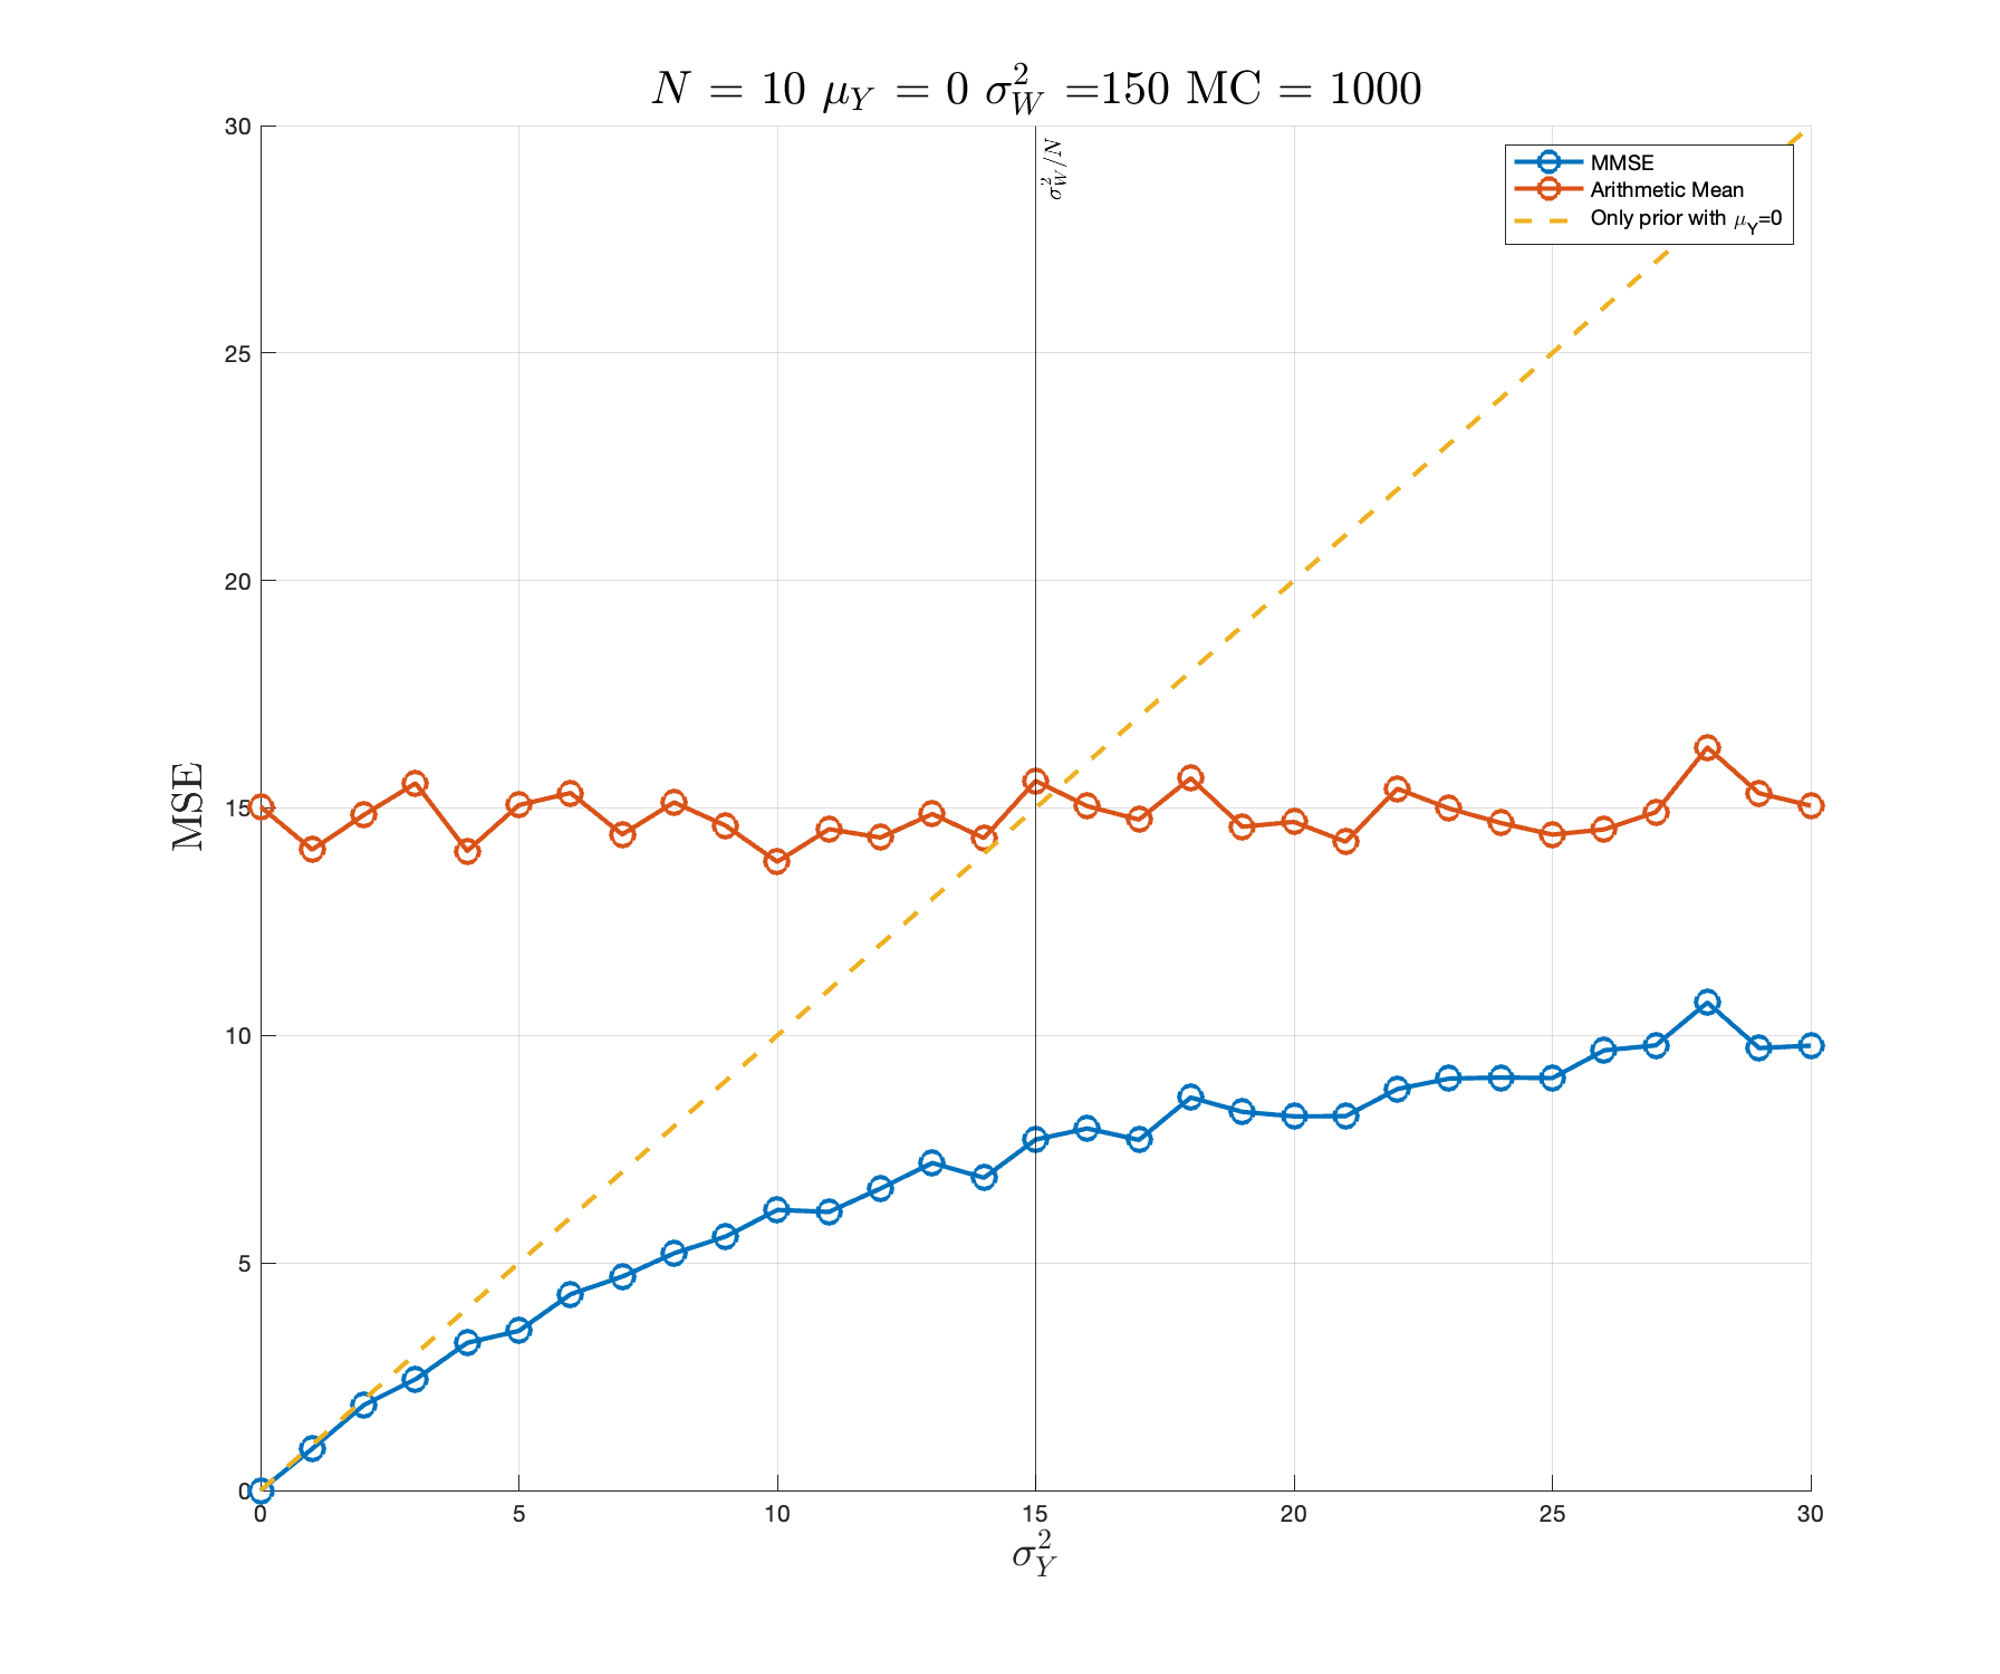
\includegraphics[width=0.8\textwidth]{./figures/appendix_a/figure_12.png}
    %\caption{MSE of the estimators $\hat Y$ and $\bar X$ as a function of $\sigma^2_Y$.}
    %\label{fig:mmse_sigma_y_small}
\end{figure}

\begin{figure}[H]
    \centering
    \begin{minipage}{0.45\textwidth}
        \centering
        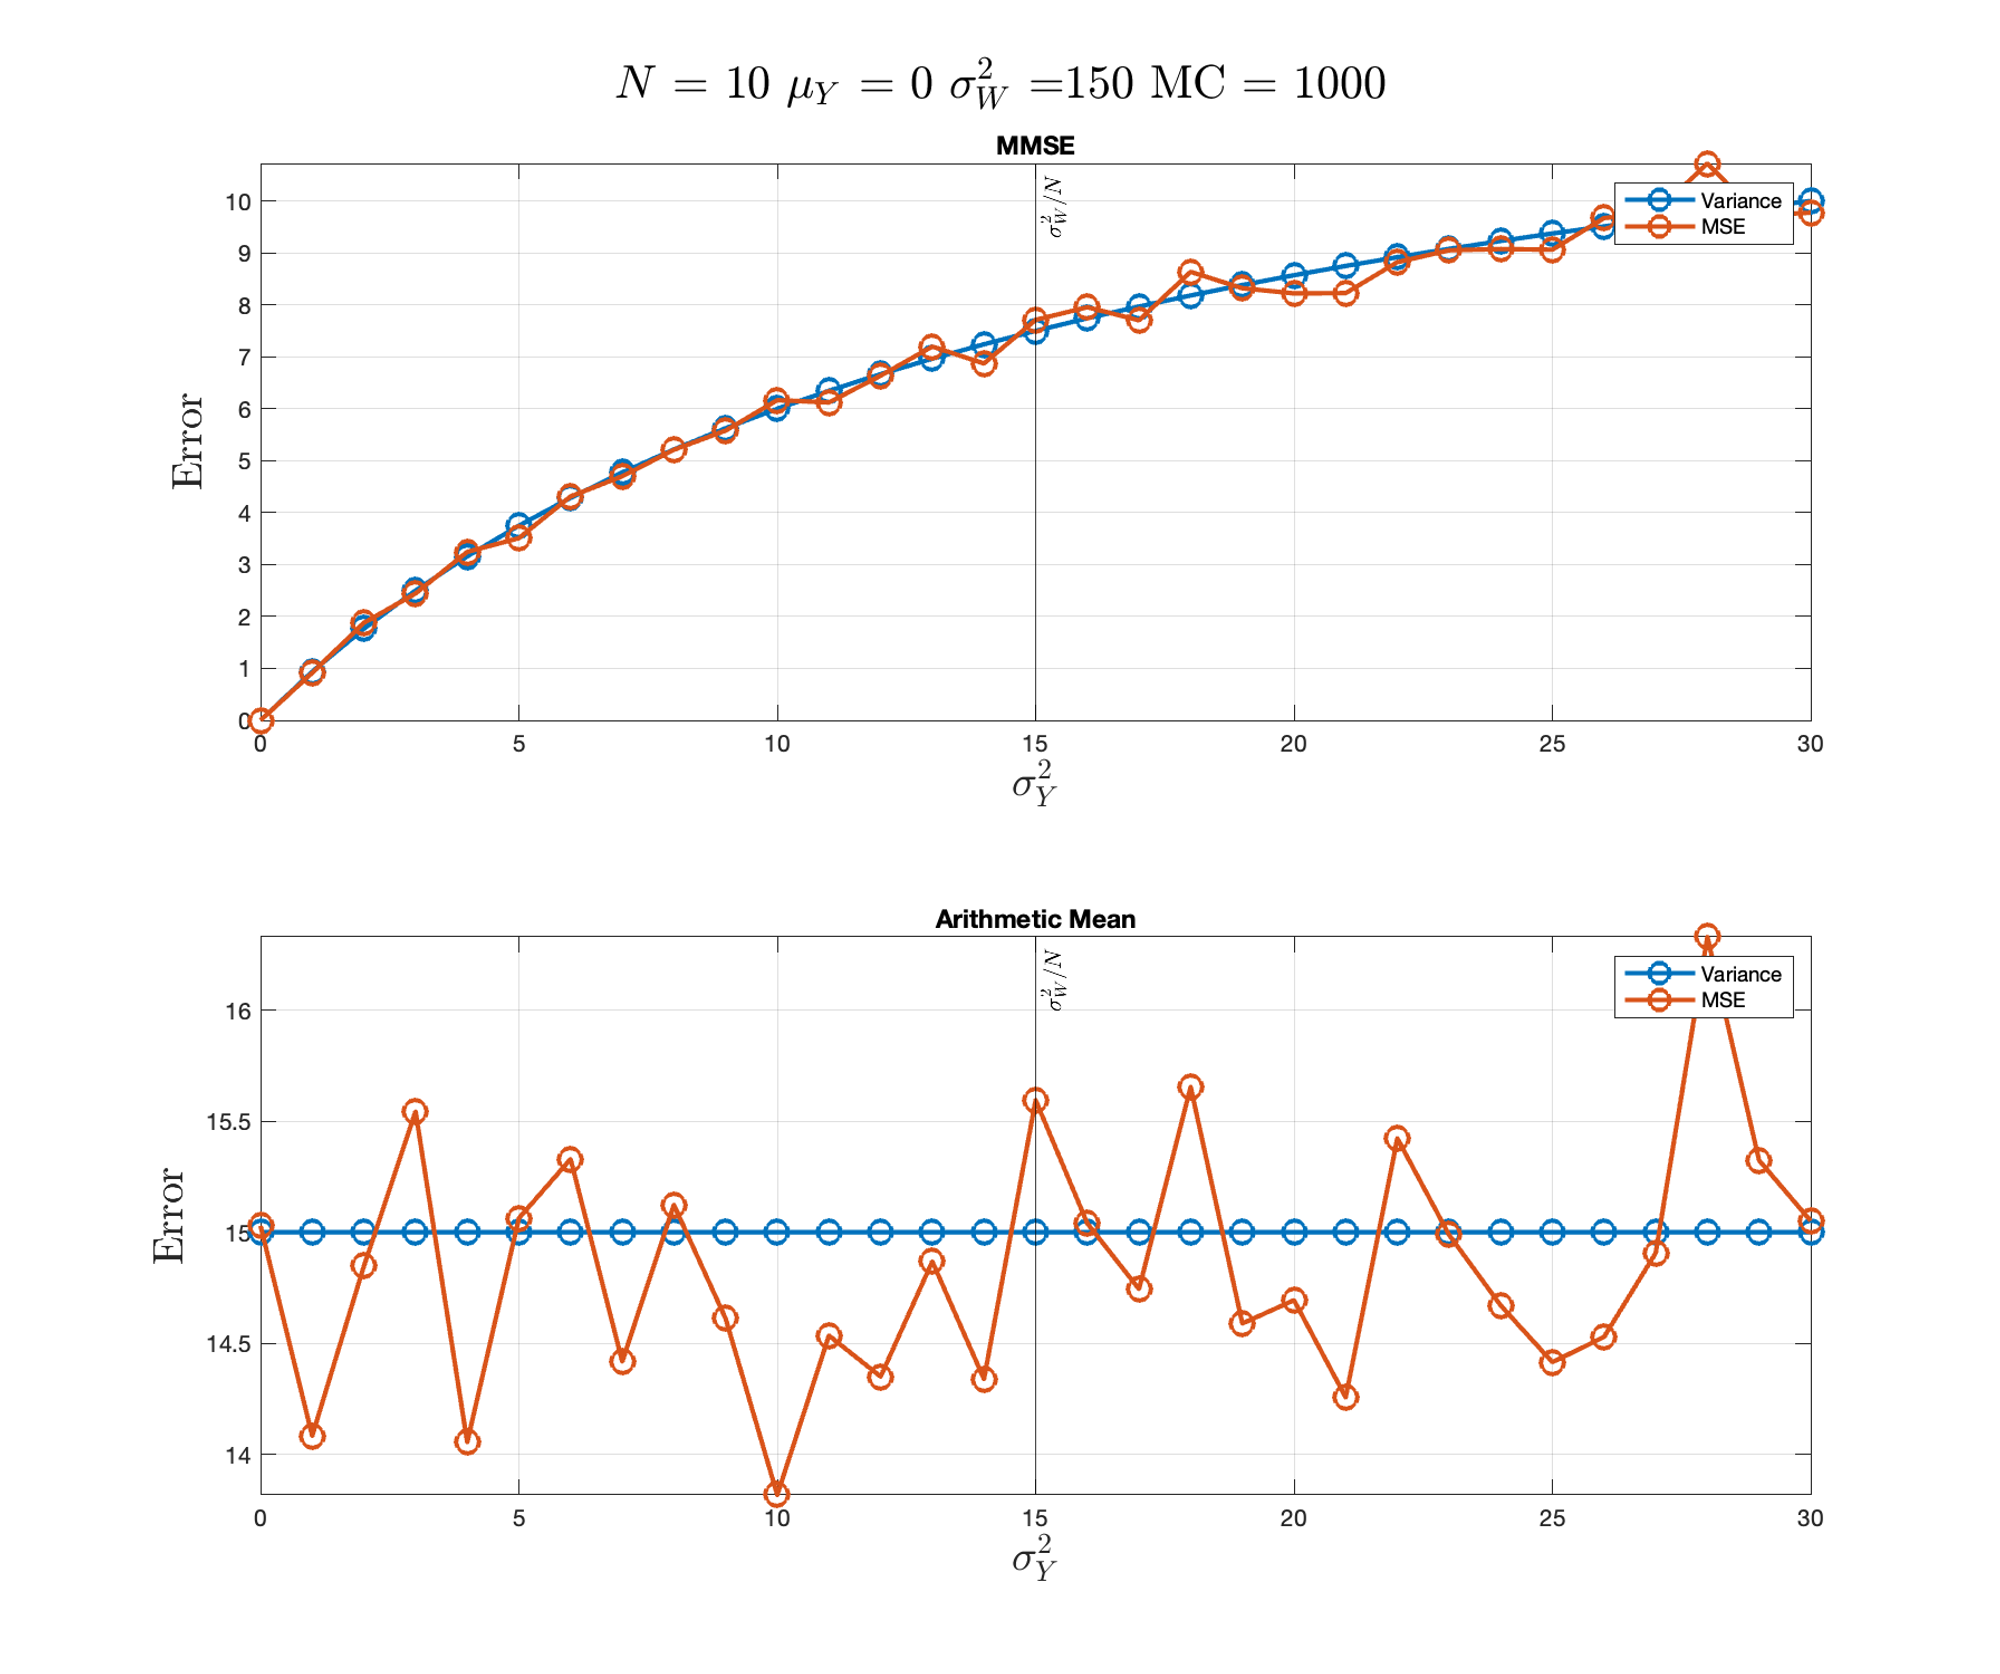
\includegraphics[width=\textwidth]{./figures/appendix_a/figure_13.png}
    \end{minipage}
    \hfill
    \begin{minipage}{0.45\textwidth}
        \centering
        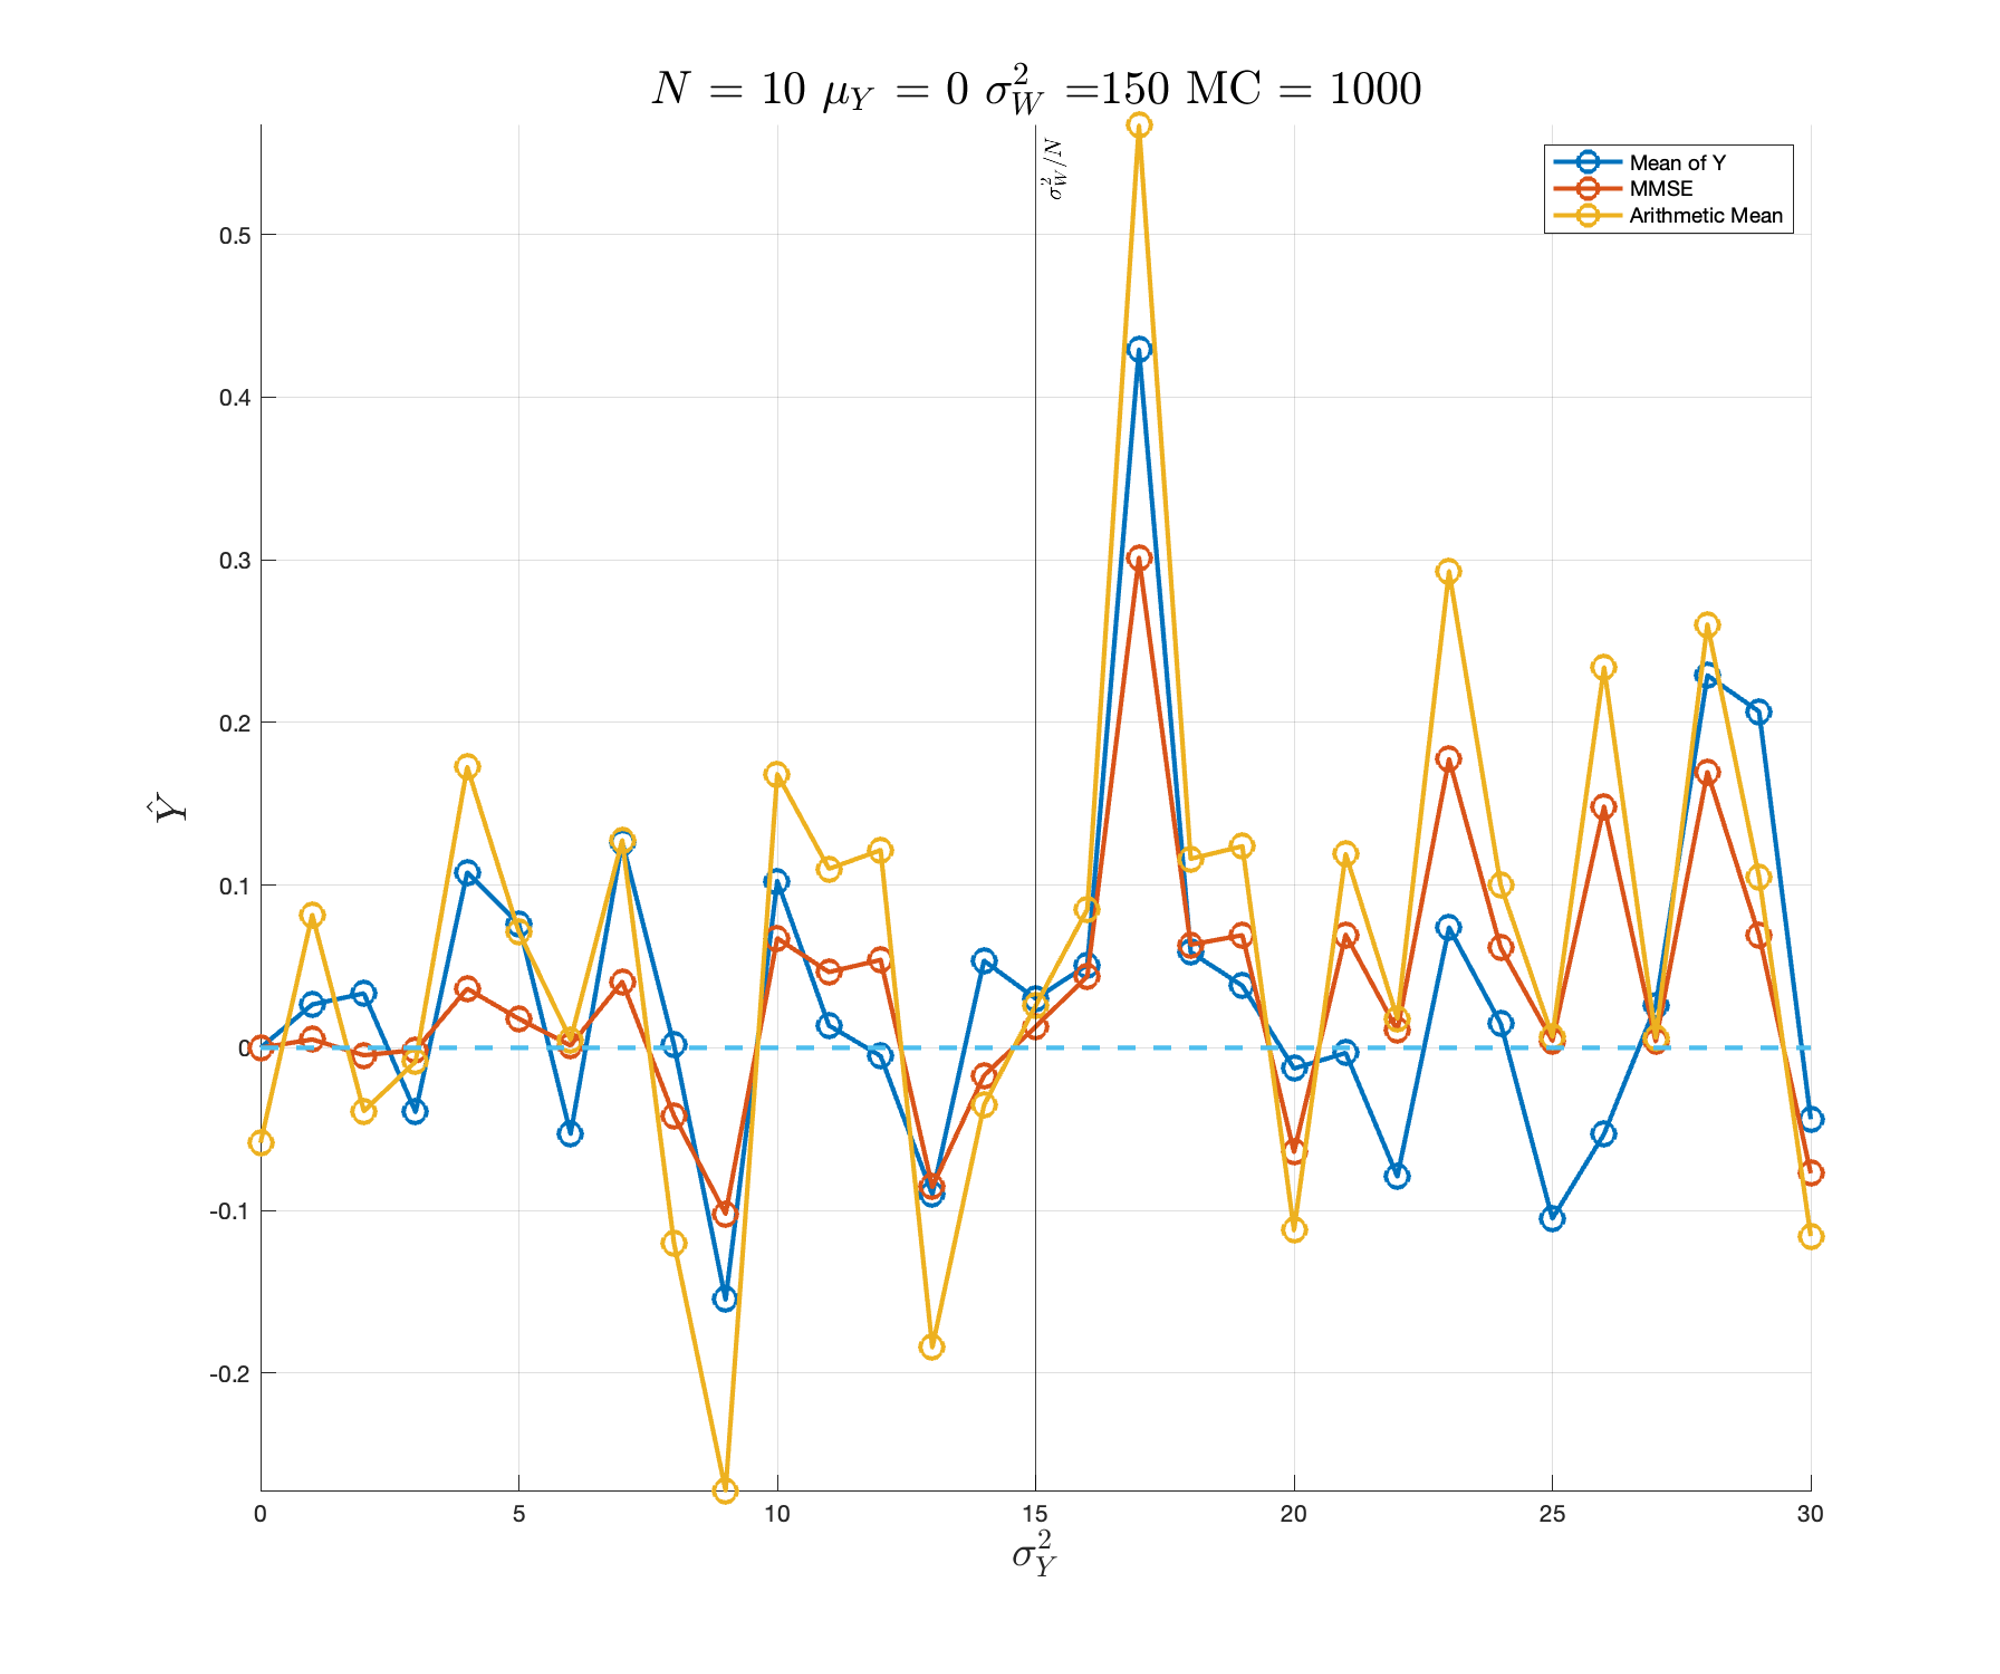
\includegraphics[width=\textwidth]{./figures/appendix_a/figure_14.png}
    \end{minipage}
    %\caption{MSE of the estimators $\hat Y$ and $\bar X$ as a function of $\sigma^2_Y$.}
    %\label{fig:mmse_sigma_y_combined}
\end{figure}

\begin{enumerate}
    \item When the two quantities oscillate around the same value, we can appreciate how the estimates made by the MMSE, compared to those made by the arithmetic mean, have the peculiarity of being closer to zero. This is because the prior information used by the MMSE indicates that the most probable values are those around the mean (specifically, zero) with a certain variance. Therefore, the estimates tend to approach the most probable values, which are around zero. And in fact, this reasoning makes sense and can be seen from the fact that the MSE calculated on the estimates of the MMSE estimator is smaller than that of the arithmetic mean.
    \item More interesting case, it shows what was said before.
    \item From this point of view, we can appreciate another thing, namely that the MSE of the arithmetic mean, net of errors due to the approximation of an expected value with a mean, is constant. This also follows from the theory:
          $$
              \mathbb E\left[\left(\frac 1N\sum X_i\right)^2\right]=\mathbb E_Y\left[\underbrace{\mathbb E_{X|Y}\left[\left(\frac 1N\sum X_i-y\right)^2\right]}_{\sigma_W^2/N}\right]
          $$
\end{enumerate}

% TODO: Non ho capito
In generale, dal valore atteso interno poiché stiamo variando la distribuzione rispetto a $X$, ma fissando un valore di $Y=y$ in generale dovremmo ottenere una funzione di $y$. In questo caso specifico il risultato non dipende da $y$. Quindi qualsiasi sia la distribuzione di $Y$, l'errore sarà sempre questo.

\begin{note}{Note}
    The fact that this error does not depend on $Y$ and the fact that $\sigma^2$ does not depend on $X$ are not related things.
\end{note}


\subsection*{Final considerations}
% TOOD: Add plot
%![Untitled](https://prod-files-secure.s3.us-west-2.amazonaws.com/62ff284d-70cf-4d0a-8be7-5596284adb1b/89954581-3456-43ea-ae34-92be37e572e0/Untitled.png)

\begin{enumerate}
    \item the theoretical error matches the error derived from the simulations
    \item the posterior mean error is always smaller than the error we would have from the prior information alone (no data). This is always more evident as we increase $\sigma^2_Y$ while the errors are similar for small values of $\sigma^2_Y$ compared to $\frac{\sigma^2 W}{N}$
    \item the MMSE error saturates to that of the arithmetic mean (likelihood estimator).
\end{enumerate}


% TODO: Add plot
%![Possiamo guardare l'asse X come indicante la qualità (migliore a dx, peggiore a sx) del dispositivo di misurazione.

%Il grafico si potrebbe migliore andando a diminuire l'asse Y.](https://prod-files-secure.s3.us-west-2.amazonaws.com/62ff284d-70cf-4d0a-8be7-5596284adb1b/490fa1ae-42ab-4fb0-8972-5b31e96cd470/Untitled.png)


\begin{enumerate}
    \item If we fixed $\sigma^2_Y$ and change $\sigma_W^2$ (and then we change the ration of this with $N$) we move from a condition ($\sigma_Y^2>\sigma^2_W/N$) where the error of the MMSE tends to the one of the arithmetic mean to a condition ($\sigma_Y^2<\sigma^2_W/N$) where the error derives from the usage of the prior information only.
    \item Thus, if we had the variance of the prior fixed, then we know how a certain variabile varies in the environment, and we had a series of measuring devices. If these devices are of \textit{low quality} we will have $\sigma_W^2$ high and then we will try to rely only on the prior information. When, instead, we have \textit{high quality} devices and a low $\sigma^2_W$ then we will tend to rely on the data.
    \item The information from the prior distribution represent the state of nature of a variabile, we can't modify them, only represent them more accurately. Then we cannot rely on $\sigma^2_W$ and on $N$. Then other than work on the quality of the devices, I can work on the quantity by increasing $N$ and buying more devices or making more independent measurement. The objective is having $\frac{\sigma^2_W}{N}$ the smaller possible.
    \item If the ration tends to infinity we will have that $\alpha \to 0$ and so the MMSE will be equal to the mean of the priori distribution that is $0$. The MSE, when approacing infinity will be equal to the error that we make when we use as estimator $0$; since $Y$ has standard deviation up to $1$, the error will be up to $1$.
\end{enumerate}

In plot \ref{fig:mse} we show the MSE with both logarithmic axes to evaluate the scaling law of the error.

% TODO: Add plot

We can see that differently from the deterministic case, the asymptotic scaling law is $\frac{1}{N}$ when $N$ is sufficiently large (and we can expect this because by increasing $N$ we go near the performances of the arithmetic mean).

There is a low that in the deterministic case tells us that the best error we can obtain follows $\frac{1}{N}$ as scaling low, but this \textit{best} estimator does not always exists.

In the bayesian case we do not have a similar rule but from this example we understood that if $N$ goes to infinity, we can except that the most important thing are the data, if we collect infinite indipendent data the prior information becomes almost irrelevant.

\section{Supervised Non Parametric Regression}
% TODO: Da sistemare
%In this exercise, we are going to use Monte Carlo simulations to verify the theoretical results obtained in the exercise \ref{sec:ex_3} and provide an analysis of the estimators $\hat f_{opt}$, $\hat f_{naive}$ and $\hat f_{knn}$ with varying parameters.
%
%Let's implement a function that computes the optimal regression function, naive kernel estimator and the nearest neighbour estimator.
%
%Let us now examine the plots.
%
%By selecting $h = 10$ the naive kernel estimator curve has degenerated into a straight line, because the interval is too large with respect to the number of samples, so the estimator just took all of the points and made the average of all the point, that is about zero because the sine is a periodic function. We actually converged to the expectation of $Y$ that is zero.
%
%On the other hand by selecting $k=10$, the nearest neighbour estimator has a shape similar to the one of the sine function.
%
%By selecting $k = 5$ and $h=0.5$, the \textit{naive estimator} starts to take some shape but it is not very similar to the optimal regression function
%% i put 10 and 0.1 much better
%
%By changing values, we observed that if $h$ is too small then we will not statisfiy the law of large numbers, and the effect is that...
%and if $k$ is too large we lose locality, and the effect is that...
%
%If H is too small i will lose law of large number => 0.01
%If K is too larg i will use locality => 50
%
%K = 50 => blue is flattered
%H = 0.01 => each point is just the sample, I am enhancing the jumps
%-> small H is similar to Knn = 1
%
%if i put K = 100 -> flat line, so i recover large
%
%small k => no LLN
%any local avg is not avg but a sample
%
%large K takes all of them but it coverges to the exeception of Y which is close of zero bc we have sin(X)
%
%0.1 and 10
%
%are we statisfied with this learned regression function
%
%we examine what happens with more samples and see if we increase we do better with other number of samples.
%
%1000 of samples
%disappointed => blue curve is not nice
%
%Knn =>
%if k remains fixed we lose LLN
%we are local but the oscillations are great
%we are not growing in term of LLN
%k must increase with N
%
%recovering LLN
%
%but there are flat => boundary effect because there are not points on the left
%
%increasing K
%increasing K
%
%we can acutally converging to the regression function
%
%
%write this code here and add the analysis of the error
%compute the error between these regression function looking at definiction
%
%montecarlo simulation
%either with a fixed training set
%or
%generate a training set each time
%
%for different size of the training set
%
%we need one law that relates k to n or h to n
%a
%$knn / n \to 0$
%$kn \to \infty$
%$1/sqrt(N)$
%
%check whether the error is going to zero
%
%check this behaviour of the plot + run simluation
%there are not theoretical values
%
%
\section{Classification}
%% TODO: 
%
%
%